\PassOptionsToPackage{table}{xcolor}
\documentclass{beamer}
% xcolor and define colors -------------------------
\usepackage[table]{xcolor}

% https://www.viget.com/articles/color-contrast/
\definecolor{purple}{HTML}{5601A4}
\definecolor{navy}{HTML}{0D3D56}
\definecolor{ruby}{HTML}{9a2515}
\definecolor{alice}{HTML}{107895}
\definecolor{daisy}{HTML}{EBC944}
\definecolor{coral}{HTML}{F26D21}
\definecolor{kelly}{HTML}{829356}
\definecolor{cranberry}{HTML}{E64173}
\definecolor{jet}{HTML}{131516}
\definecolor{asher}{HTML}{555F61}
\definecolor{slate}{HTML}{314F4F}

% Mixtape Sessions
\definecolor{picton-blue}{HTML}{00b7ff}
\definecolor{violet-red}{HTML}{ff3881}
\definecolor{sun}{HTML}{ffaf18}
\definecolor{electric-violet}{HTML}{871EFF}

% Main theme colors
\definecolor{accent}{HTML}{00b7ff}
\definecolor{accent2}{HTML}{871EFF}
\definecolor{gray100}{HTML}{f3f4f6}
\definecolor{gray800}{HTML}{1F292D}

\definecolor{bgRaspberry}{HTML}{ff96a9}
\definecolor{bgCranberry}{HTML}{fda4d0}
\definecolor{bgOrange}{HTML}{f6b97b}
\definecolor{bgPurple}{HTML}{adb4f4}
\definecolor{bgBlue}{HTML}{cdfbff}
\definecolor{bgGreen}{HTML}{8ee7af}
\definecolor{bgRose}{HTML}{fecdd4}
\definecolor{bgYellow}{HTML}{ffea88}

% Beamer Options -------------------------------------

% Background
\setbeamercolor{background canvas}{bg = white}

% Change text margins
\setbeamersize{text margin left = 15pt, text margin right = 15pt}

% \alert
\setbeamercolor{alerted text}{fg = accent2}

% Frame title
\setbeamercolor{frametitle}{bg = white, fg = jet}
\setbeamercolor{framesubtitle}{bg = white, fg = accent}
\setbeamerfont{framesubtitle}{size = \small, shape = \itshape}

% Block
\setbeamercolor{block title}{fg = white, bg = accent2}
\setbeamercolor{block body}{fg = gray800, bg = gray100}

% Title page
\setbeamercolor{title}{fg = gray800}
\setbeamercolor{subtitle}{fg = accent}

%% Custom \maketitle and \titlepage
\setbeamertemplate{title page}
{
    %\begin{centering}
        \vspace{20mm}
        {\Large \usebeamerfont{title}\usebeamercolor[fg]{title}\inserttitle}\\
        {\large \itshape \usebeamerfont{subtitle}\usebeamercolor[fg]{subtitle}\insertsubtitle}\\ \vspace{10mm}
        {\insertauthor}\\
        {\color{asher}\small{\insertdate}}\\
    %\end{centering}
}

% Table of Contents
\setbeamercolor{section in toc}{fg = accent!70!jet}
\setbeamercolor{subsection in toc}{fg = jet}

% Button
\setbeamercolor{button}{bg = accent}

% Remove navigation symbols
\setbeamertemplate{navigation symbols}{}

% Table and Figure captions
\setbeamercolor{caption}{fg=jet!70!white}
\setbeamercolor{caption name}{fg=jet}
\setbeamerfont{caption name}{shape = \itshape}

% Bullet points

%% Fix left-margins
\settowidth{\leftmargini}{\usebeamertemplate{itemize item}}
\addtolength{\leftmargini}{\labelsep}

%% enumerate item color
\setbeamercolor{enumerate item}{fg = accent}
\setbeamerfont{enumerate item}{size = \small}
\setbeamertemplate{enumerate item}{\insertenumlabel.}

%% itemize
\setbeamercolor{itemize item}{fg = accent!70!white}
\setbeamerfont{itemize item}{size = \small}
\setbeamertemplate{itemize item}[circle]

%% right arrow for subitems
\setbeamercolor{itemize subitem}{fg = accent!60!white}
\setbeamerfont{itemize subitem}{size = \small}
\setbeamertemplate{itemize subitem}{$\rightarrow$}

\setbeamertemplate{itemize subsubitem}[square]
\setbeamercolor{itemize subsubitem}{fg = jet}
\setbeamerfont{itemize subsubitem}{size = \small}


% Special characters

\usepackage{collectbox}

\makeatletter
\newcommand{\mybox}{%
    \collectbox{%
        \setlength{\fboxsep}{1pt}%
        \fbox{\BOXCONTENT}%
    }%
}
\makeatother





% Links ----------------------------------------------

\usepackage{hyperref}
\hypersetup{
  colorlinks = true,
  linkcolor = accent2,
  filecolor = accent2,
  urlcolor = accent2,
  citecolor = accent2,
}


% Line spacing --------------------------------------
\usepackage{setspace}
\setstretch{1.1}


% \begin{columns} -----------------------------------
\usepackage{multicol}


% Fonts ---------------------------------------------
% Beamer Option to use custom fonts
\usefonttheme{professionalfonts}

% \usepackage[utopia, smallerops, varg]{newtxmath}
% \usepackage{utopia}
\usepackage[sfdefault,light]{roboto}

% Small adjustments to text kerning
\usepackage{microtype}



% Remove annoying over-full box warnings -----------
\vfuzz2pt
\hfuzz2pt


% Table of Contents with Sections
\setbeamerfont{myTOC}{series=\bfseries, size=\Large}
\AtBeginSection[]{
        \frame{
            \frametitle{Roadmap}
            \tableofcontents[current]
        }
    }


% Tables -------------------------------------------
% Tables too big
% \begin{adjustbox}{width = 1.2\textwidth, center}
\usepackage{adjustbox}
\usepackage{array}
\usepackage{threeparttable, booktabs, adjustbox}

% Fix \input with tables
% \input fails when \\ is at end of external .tex file
\makeatletter
\let\input\@@input
\makeatother

% Tables too narrow
% \begin{tabularx}{\linewidth}{cols}
% col-types: X - center, L - left, R -right
% Relative scale: >{\hsize=.8\hsize}X/L/R
\usepackage{tabularx}
\newcolumntype{L}{>{\raggedright\arraybackslash}X}
\newcolumntype{R}{>{\raggedleft\arraybackslash}X}
\newcolumntype{C}{>{\centering\arraybackslash}X}

% Figures

% \imageframe{img_name} -----------------------------
% from https://github.com/mattjetwell/cousteau
\newcommand{\imageframe}[1]{%
    \begin{frame}[plain]
        \begin{tikzpicture}[remember picture, overlay]
            \node[at = (current page.center), xshift = 0cm] (cover) {%
                \includegraphics[keepaspectratio, width=\paperwidth, height=\paperheight]{#1}
            };
        \end{tikzpicture}
    \end{frame}%
}

% subfigures
\usepackage{subfigure}


% Highlight slide -----------------------------------
% \begin{transitionframe} Text \end{transitionframe}
% from paulgp's beamer tips
\newenvironment{transitionframe}{
    \setbeamercolor{background canvas}{bg=accent!40!black}
    \begin{frame}\color{accent!10!white}\LARGE\centering
}{
    \end{frame}
}


% Table Highlighting --------------------------------
% Create top-left and bottom-right markets in tabular cells with a unique matching id and these commands will outline those cells
\usepackage[beamer,customcolors]{hf-tikz}
\usetikzlibrary{calc, fit, shadows, arrows, arrows.meta, shapes.misc, shapes,decorations, decorations.pathreplacing, positioning}
\usepackage[most,skins]{tcolorbox}
\tcbuselibrary{breakable}
\tcbset{
  highlight math/.style={
    notitle, enhanced,
    on line, boxsep=2pt, left=0pt, right=0pt, top=0pt, bottom=0pt,
    colback = bgRaspberry, colframe = white,
  }
}

% To set the hypothesis highlighting boxes red.
\newcommand\marktopleft[1]{%
    \tikz[overlay,remember picture]
        \node (marker-#1-a) at (0,1.5ex) {};%
}
\newcommand\markbottomright[1]{%
    \tikz[overlay,remember picture]
        \node (marker-#1-b) at (0,0) {};%
    \tikz[accent!80!jet, ultra thick, overlay, remember picture, inner sep=4pt]
        \node[draw, rectangle, fit=(marker-#1-a.center) (marker-#1-b.center)] {};%
}


% Define custom slide coordinate system ----------------------------------------
% https://tex.stackexchange.com/questions/89588/positioning-relative-to-page-in-tikz
% Defining a new coordinate system for the page:
%
% ┌──────────────────────────────────────────────┐
% │ (0, 0)                                (1, 0) │
% │                                              │
% │                                              │
% │                                              │
% │                                              │
% │                                              │
% │ (0, 1)                                (1, 1) │
% └──────────────────────────────────────────────┘
%
% source: https://tex.stackexchange.com/questions/89588/positioning-relative-to-page-in-tikz
%
\makeatletter
\def\parsecomma#1,#2\endparsecomma{\def\page@x{#1}\def\page@y{#2}}
\tikzdeclarecoordinatesystem{page}{
    \parsecomma#1\endparsecomma
    \pgfpointanchor{current page}{north west}
    % Save the upper left corner
    \pgf@xa=\pgf@x%
    \pgf@ya=\pgf@y%
    % save the lower right corner
    \pgfpointanchor{current page}{south east}
    \pgf@xb=\pgf@x%
    \pgf@yb=\pgf@y%
    % Transform to the correct placement
    \pgfmathparse{(\pgf@xb-\pgf@xa)*\page@x+\pgf@xa}
    \expandafter\pgf@x\expandafter=\pgfmathresult pt
    \pgfmathparse{(\pgf@yb-\pgf@ya)*\page@y+\pgf@ya}
    \expandafter\pgf@y\expandafter=\pgfmathresult pt
}
\makeatother

% To overlay on beamer slides, use the following:
%
% \begin{tikzpicture}[remember picture, overlay]
%   \node[anchor = north west] (anchor_name) at (page cs:0.0, 0.0) {
%     CONTENT HERE
%   };
% \end{tikzpicture}
%
% Note page cs is the coordinate system from above

% To help with placement, I will use `\devgrid` on a slide to figure out the coordinates of `page cs` to the 0.1
\newcommand{\devgrid}{
  \begin{tikzpicture}[remember picture, overlay]
    % vertical lines
    \draw (page cs: 0.1, 0.0) edge[black!20!white, line width = 0.3mm, dotted] (page cs: 0.1, 1.0);
    \draw (page cs: 0.2, 0.0) edge[black!20!white, line width = 0.3mm, dotted] (page cs: 0.2, 1.0);
    \draw (page cs: 0.3, 0.0) edge[black!20!white, line width = 0.3mm, dotted] (page cs: 0.3, 1.0);
    \draw (page cs: 0.4, 0.0) edge[black!20!white, line width = 0.3mm, dotted] (page cs: 0.4, 1.0);
    \draw (page cs: 0.5, 0.0) edge[black!20!white, line width = 0.3mm, dotted] (page cs: 0.5, 1.0);
    \draw (page cs: 0.6, 0.0) edge[black!20!white, line width = 0.3mm, dotted] (page cs: 0.6, 1.0);
    \draw (page cs: 0.7, 0.0) edge[black!20!white, line width = 0.3mm, dotted] (page cs: 0.7, 1.0);
    \draw (page cs: 0.8, 0.0) edge[black!20!white, line width = 0.3mm, dotted] (page cs: 0.8, 1.0);
    \draw (page cs: 0.9, 0.0) edge[black!20!white, line width = 0.3mm, dotted] (page cs: 0.9, 1.0);

    % horizontal lines
    \draw (page cs: 0.0, 0.1) edge[black!20!white, line width = 0.3mm, dotted] (page cs: 1.0, 0.1);
    \draw (page cs: 0.0, 0.2) edge[black!20!white, line width = 0.3mm, dotted] (page cs: 1.0, 0.2);
    \draw (page cs: 0.0, 0.3) edge[black!20!white, line width = 0.3mm, dotted] (page cs: 1.0, 0.3);
    \draw (page cs: 0.0, 0.4) edge[black!20!white, line width = 0.3mm, dotted] (page cs: 1.0, 0.4);
    \draw (page cs: 0.0, 0.5) edge[black!20!white, line width = 0.3mm, dotted] (page cs: 1.0, 0.5);
    \draw (page cs: 0.0, 0.6) edge[black!20!white, line width = 0.3mm, dotted] (page cs: 1.0, 0.6);
    \draw (page cs: 0.0, 0.7) edge[black!20!white, line width = 0.3mm, dotted] (page cs: 1.0, 0.7);
    \draw (page cs: 0.0, 0.8) edge[black!20!white, line width = 0.3mm, dotted] (page cs: 1.0, 0.8);
    \draw (page cs: 0.0, 0.9) edge[black!20!white, line width = 0.3mm, dotted] (page cs: 1.0, 0.9);
  \end{tikzpicture}
}

\usepackage{breqn} % Breaks lines

\usepackage{amsmath}
\usepackage{mathtools}

\usepackage{pdfpages} % \includepdf
\usepackage{listings} % R code
\usepackage{verbatim} % verbatim

% Video stuff
\usepackage{media9}

% packages for bibs and cites
\usepackage{natbib}
\usepackage{har2nat}
\newcommand{\possessivecite}[1]{\citeauthor{#1}'s \citeyearpar{#1}}
\usepackage{breakcites}
\usepackage{alltt}

% Setup math operators
\DeclareMathOperator{\E}{E} \DeclareMathOperator{\tr}{tr} \DeclareMathOperator{\se}{se} \DeclareMathOperator{\I}{I} \DeclareMathOperator{\sign}{sign} \DeclareMathOperator{\supp}{supp} \DeclareMathOperator{\plim}{plim}
\DeclareMathOperator*{\dlim}{\mathnormal{d}\mkern2mu-lim}
\newcommand\independent{\protect\mathpalette{\protect\independenT}{\perp}}
   \def\independenT#1#2{\mathrel{\rlap{$#1#2$}\mkern2mu{#1#2}}}
\newcommand*\colvec[1]{\begin{pmatrix}#1\end{pmatrix}}

\newcommand{\myurlshort}[2]{\href{#1}{\textcolor{gray}{\textsf{#2}}}}


\begin{document}

\begin{frame}[plain]  % Removes header/footer and gives you full vertical control
\vfill
\begin{center}
  
\includegraphics[width=0.85\linewidth]{./lecture_includes/banner_cropped}
\end{center}
\vfill
\end{frame}





\section{Violations of Parallel Trends}

\subsection{Event Study Plots}

\begin{frame}{Different parallel trends assumptions}

\begin{itemize}
\item Covariates serve very different purposes with diff-in-diff than with cross-sectional regressions
\item "Omitted variable bias" is not about dealing with future endogeneities, but with imbalanced covariates that cause trends in missing potential outcomes\item When parallel trends holds from baseline, then:
	\begin{enumerate}
	\item Unconditional parallel trends: no covariates needed
	\item Conditional parallel trends: covariates needed
	\end{enumerate}
\item And even then we have a different parallel trends for the imputation estimators that requires it hold in every pre and post period
\end{itemize}
\end{frame}

\begin{frame}{Unconditional Parallel Trends}

\begin{itemize}
\item Unconditional parallel trends is a 2x2 on $\Delta E[Y^0]$ which satisfies:
	$$\textcolor{red}{\Delta E[Y^0|D=1]} - \Delta E[Y^0|D=0] = 0$$
\item Unconditional parallel trends is very close to assuming that the the treatment was as good as random since it is randomness that tends to set mean potential outcomes equal across treatment status
\item Very often misinterpreted, also, as it is in not testable, even with event studies
\end{itemize}


\end{frame}

\begin{frame}{Intuition behind event studies}

\begin{itemize}

	\item Pre-period falsifications are common in causal inference, even outside of diff-in-diff, because the pre-period probably has the same confounder structure, but no treatment (Imbens regularly suggests it even outside of panel methods -- see Imbens and Xu 2024)
	\item In that spirit, event studies grew up as a basic falsification to illustrate that if groups were similar on trends in the past, they'd likely be similar on trends in the future, even if past trends are not the same as future trends
	\item But event studies require more than two periods and therefore we call it the 2xT design (Baker, et al. 2025)


\end{itemize}

\end{frame}




\begin{frame}{Three Different Falsification Strategies}

	\begin{enumerate}
	\item \textbf{Event study falsification \#1}: diff-in-diff applied to the past which under NA is only estimating a parallel trend
	\item \textbf{Same outcome, different group falsification \#2}: diff-in-diff applied to same outcomes, but similar and untreated group with similar confounder structure
	\item \textbf{Different group, same outcome falsification \#3}: diff-in-diff applied to different and implausible outcomes with similar confounder structures using the same groups
	\end{enumerate}


\end{frame}






\begin{frame}{Event study regression}

 $$Y_{its} = \alpha + \sum_{\tau=-2}^{-q}\mu_{\tau} (D_s \times \tau_t) + \sum_{\tau=0}^m\delta_{\tau} (D_s \times \tau_t) + \tau_t + D_s + \varepsilon_{ist}$$
		\begin{itemize}
		\item With a simple 2x2, you are interacting treatment indicator with calendar year dummies
		\item Includes $q$ leads (dropping the $t-1$ as baseline) and $m$ lags
		\item Since treatment did not happen until $\tau=0$, then pre-treatment coefficients only capture differential trends
		\end{itemize}
\end{frame}

\begin{frame}{Reviewing previous slide for emphasis}


\begin{itemize}
\item Under NA, SUTVA and parallel pre-trends, then mechanically $\widehat{\mu_{\tau}}$ will be zero as everything cancels out
	\begin{itemize}
\item There are still specification and power issues that Jon Roth has written about, but I will skip that
	\end{itemize}
\item But also under NA, SUTVA and parallel trends (post trends), then $\widehat{\delta}$ are estimates of the ATT at points in time
\item  Typically you'll plot the coefficients and 95\% CI on all leads and lags
\end{itemize}

\end{frame}

\begin{frame}{Normal DiD coefficient}

\begin{eqnarray*}
\widehat{\delta} &=& \underbrace{E[Y^1_k | Post] - \textcolor{red}{E[Y^0_k | Post]}}_{\mathclap{\text{Post-treatment ATT}}} \\
&& + \bigg [  \underbrace{\textcolor{red}{E[Y^0_k | Post]} - E[Y^0_k | Pre] \bigg ] - \bigg [ E[Y^0_U | Post] - E[Y_U^0 | Pre] }_{\mathclap{\text{Post treatment differential trends}}} \bigg ]
\end{eqnarray*}


\begin{itemize}
\item 2x2 diff-in-diff \emph{always} equals the sum of those under NA and an untreated comparison group
\item It even equals that in the pre-period -- it's an identity
\end{itemize}



\end{frame}

\begin{frame}{Pre-treatment DiD coefficient}

\begin{eqnarray*}
\widehat{\delta}_{t-2} &=& \underbrace{E[Y^1_k | t-2] - \textcolor{red}{E[Y^0_k | t-2]}}_{\mathclap{\text{ATT = 0 under NA}}} \\
&& + \underbrace{\bigg[ E[Y^0_k | t-2] - E[Y^0_k | Pre] \bigg] - \bigg[ E[Y^0_U | t-2] - E[Y^0_U | Pre] \bigg]}_{\mathclap{\text{Differential pre-trends}}}
\end{eqnarray*}
\bigskip

\begin{itemize}
\item Recall NA means $Y=Y^0$ for all pre-periods, or $\delta_{t<0}=0$
\item Since every event study is a simple 2x2, then pre-treatment event study coefficients \emph{only} measure pre-trends
\end{itemize}


\end{frame}




\begin{frame}{Medicaid and Affordable Care Act example}

\begin{figure}
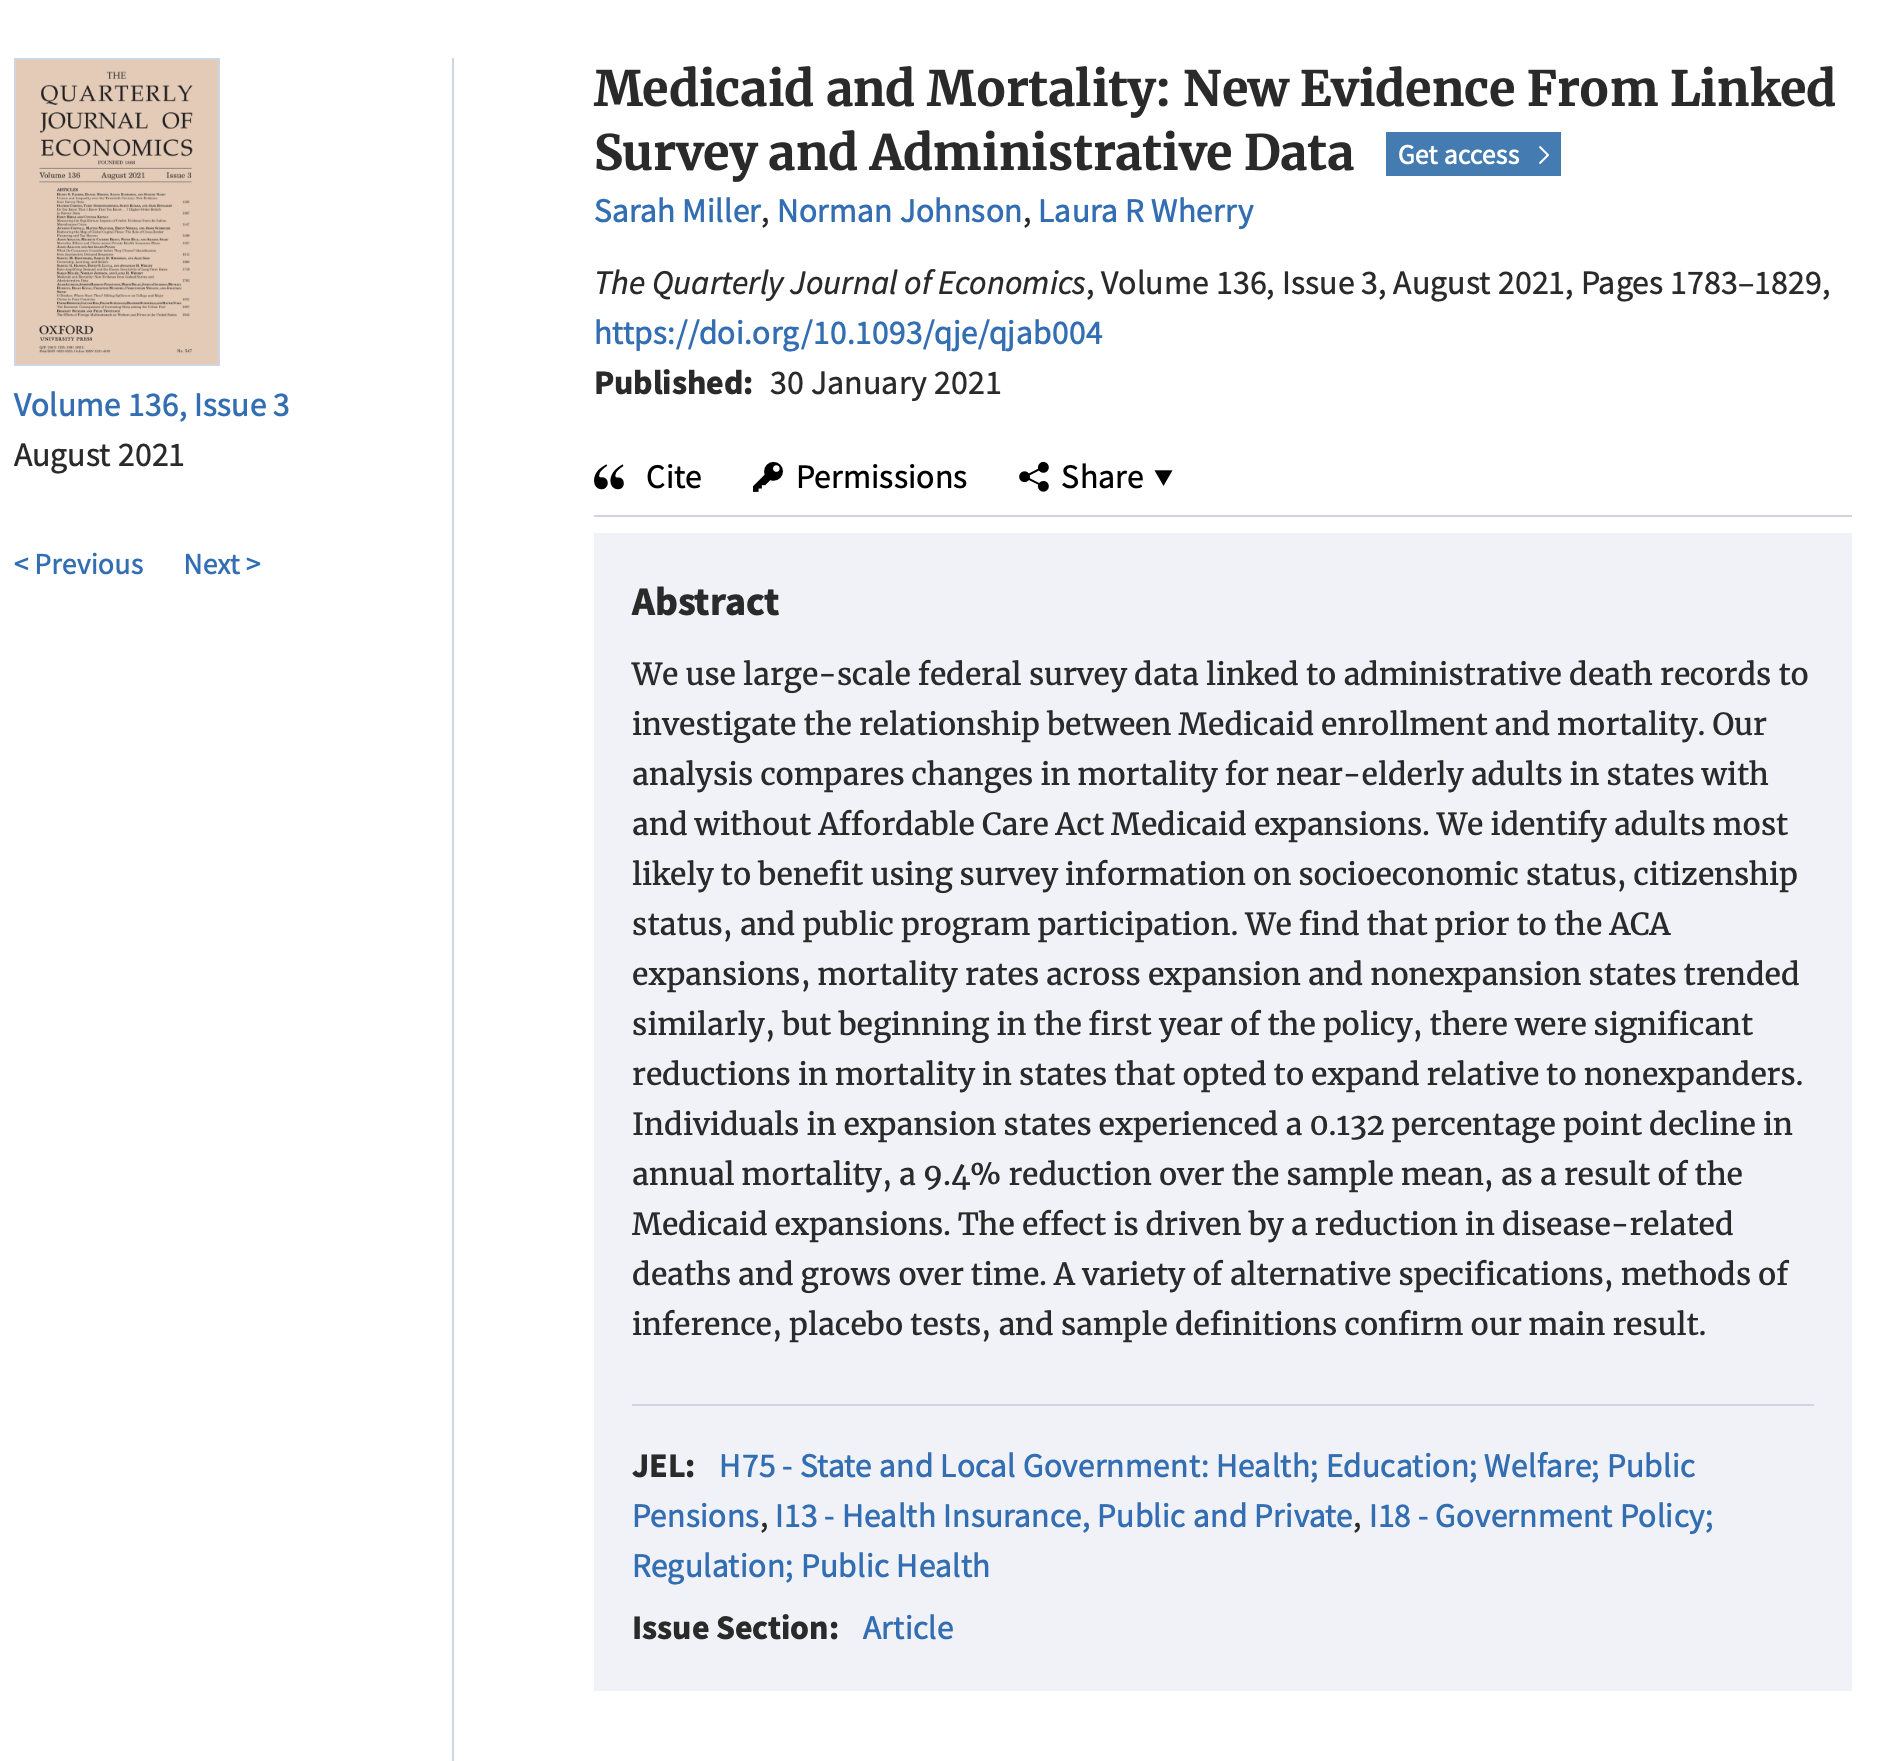
\includegraphics[scale=0.25]{./lecture_includes/medicaid_qje}
\end{figure}

\end{frame}


\begin{frame}{Evidence versus Results}

\begin{itemize}
\item High quality linked administrative data showing rewards to accessing new data -- but still only a diff-in-diff
\item Has five elements that I want to guide us through:
	\begin{enumerate}
	\item Bite -- show the first order effects (e.g., the program was adopted)
	\item Falsifications -- same outcome/different groups and/or different group/same outcome
	\item Event study -- best event study graphs are pre-treatment zeroes with small confidence intervals (will need power)
	\item Main results -- simple summaries to aid interpretation (consider using baseline mean for treatment)
	\item Mechanisms -- test your conjectures with more data (don't just tell stories)
	\end{enumerate}
\item Here's a selected summary of their study in light of those 5 elements
\end{itemize}

\end{frame}



\begin{frame}{Evidence versus Results}

\begin{itemize}
\item \textbf{Bite} -- Medicaid expansion shifted people into Medicaid and out of uninsured status
\item \textcolor{black}{\textbf{Falsifications}} -- No effect of Medicaid on a similar group that didn't enroll
\item \textbf{Event study} and \textbf{Main results} -- Mostly compelling dynamic event study coefficients on near elderly mortality and simple summary (comparing to sample mean)
\item \textcolor{black}{\textbf{Mechanisms}} --  Disease-related mortality declines that compound over time
\end{itemize}

\end{frame}

\begin{frame}{Bite}

\begin{itemize}
\item Imagine if your main results were shown but someone else found that no one ever got on the program you're studying -- seems implausible a program can work if no one uses it?
\item Bite in this context means that when US states made Medicaid more generous, people got on Medicaid who would not have been on it otherwise
\item Not always possible, but I think you want to push yourself to find the data that can support bite until you just feel the data does not exist (but keep trying anyway)
\end{itemize}

\end{frame}


\imageframe{./lecture_includes/Miller_Medicaid1.png}

\imageframe{./lecture_includes/Miller_Medicaid2.png}

\imageframe{./lecture_includes/Miller_Medicaid3.png}


\begin{frame}{Falsification}

\begin{itemize}

\item Their study focuses on ``near elderly'', which means just under 65
\item They choose just under 65 because in the US, 65 and older are eligible for Medicare so more generous Medicaid is irrelevant
\item \emph{But} probably the near elderly and the elderly are equally susceptible to unobserved factors correlated with the treatment
\item So they painstakingly examine the effects on elderly as a falsification as this will strengthen the parallel trends assumption on the near elderly
\end{itemize}

\end{frame}

\begin{frame}{Falsifications on elderly}

	\begin{figure}
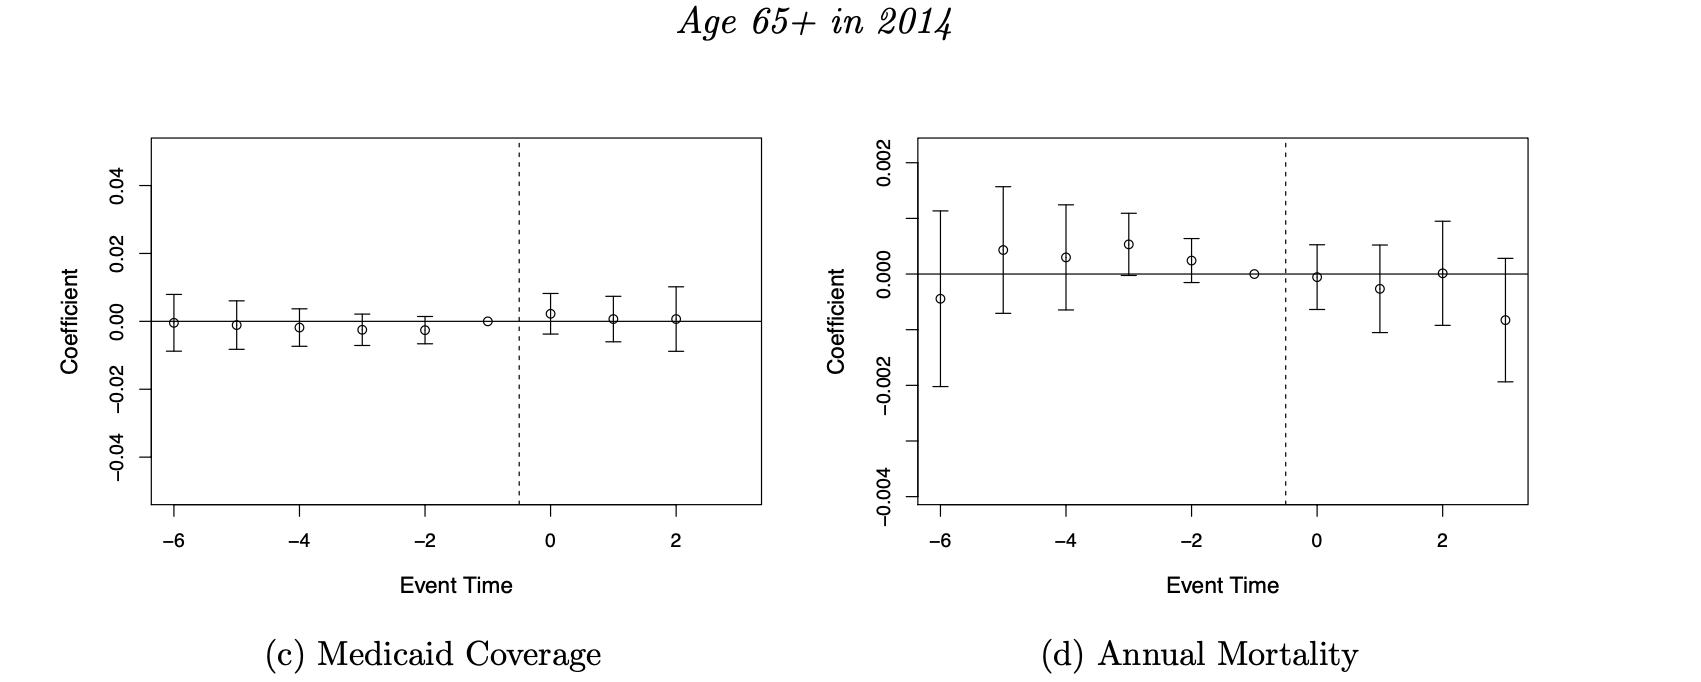
\includegraphics[scale=0.425]{./lecture_includes/placebo_medicaid}
	\end{figure}

\end{frame}

\begin{frame}{Main result}

\begin{itemize}

\item Finally they focus on the main result -- and there's more in the paper than I'm showing
\item Event study plots with same specification as the rest allowing us to look at the pre-trends and the post-treatment coefficients
\item If parallel trends holds, then the post-treatment coefficients are interpreted as ATT parameter estimates for each time period
\item The result alone isn't nearly as strong the result in combination with the rest, but it could still be wrong as parallel trends is ultimately not verfiable
\end{itemize}

\end{frame}



\begin{frame}{Near elderly mortality and Medicaid expansion}

	\begin{figure}
	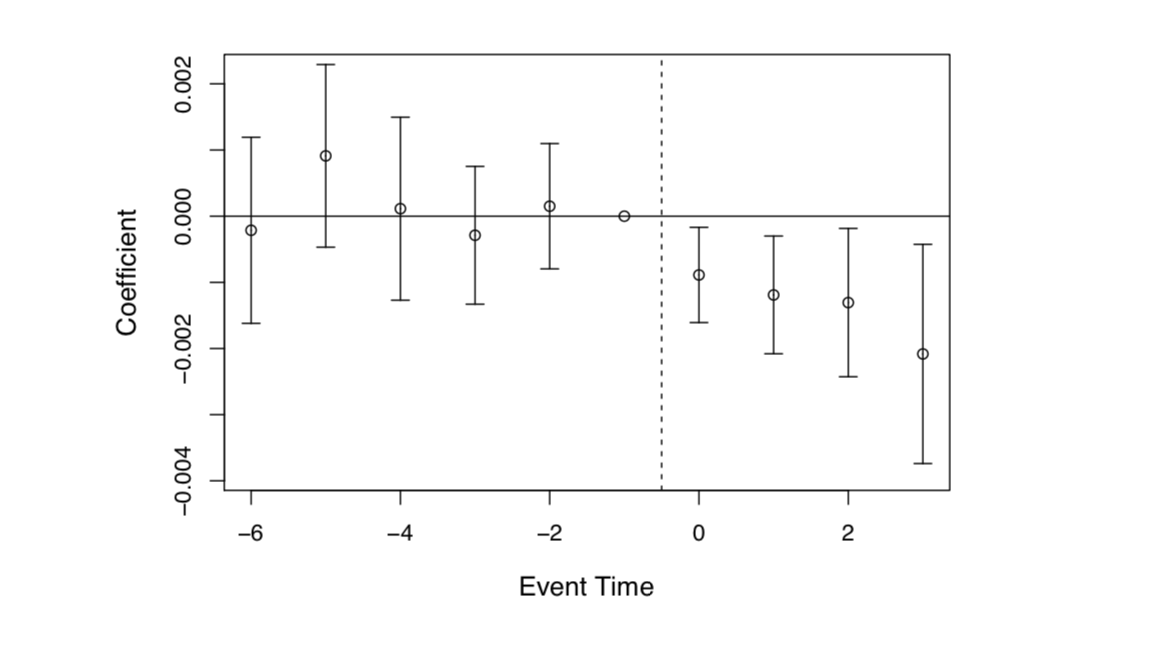
\includegraphics[scale=0.3]{./lecture_includes/Miller_Medicaid4.png}
	\end{figure}

\end{frame}

\begin{frame}{Summarizing evidence and results}

\begin{itemize}
\item \textbf{Bite}: Increases in enrollment and reductions in uninsured support that there is adoption of the treatment
\item \textbf{Event studies}: Compelling graphics showing similarities between treatment and control
\item \textbf{Falsifications}: no effect on a similar group who isn't eligible
\item \textcolor{black}{Main results}: Simplified result is "9.2\% reduction in mortality among the near-elderly" using sample means (very common to do this)
\item \textcolor{black}{Mechanism}: ``The effect is driven by a reduction in disease-related deaths and grows over time.''
\end{itemize}

\end{frame}

\begin{frame}{Making event study}

\begin{itemize}
\item When there is only one treatment group and one comparison group, then you run a regression with an interaction of the treatment group dummy and the calendar year dummies (plus both separately)
\item You must drop $t-\tau$ as the baseline (e.g., $t-1$) and it must be $Y^0$ untreated comparisons (No Anticipation)
\item When you drop $t-\tau$ as the baseline, then all estimates become "long differences" compared to that point
\end{itemize}

\end{frame}




\subsection{Other Falsifications}

\begin{frame}{Proof vs Evidence}

\begin{itemize}
\item Think of event studies as \emph{evidence}, not \emph{proof}
	\begin{itemize}
	\item Prosecutor based on police produces fingerprints, eyewitnesses and imprints in mud
	\end{itemize}
\item Event studies are evidence of pre-trends only, but they do not protect against bias caused by policies or events that happen simultaneous to the treatment
	\begin{itemize}
	\item When policies happen at the same as the treatment which affect $Y^0$, then parallel trends is violated by definition
	\item But maybe there is a way to test for this using falsifications
	\end{itemize}
\item Falsifications are designed to rule out the possibility that the estimated treatment effects were caused by something else -- but you need some ideas of what those might be
\end{itemize}
\end{frame}

\begin{frame}{Two types of falsifications}

\begin{enumerate}
\item Same outcome as your main model, but using an untreated group
	\begin{itemize}
	\item Run your main model on a group that shouldn’t respond to treatment.
	\item If your estimate is still large, something else might be driving the results.
	\end{itemize}
\item Same treatment group with an unlikely outcome
	\begin{itemize}
	\item Think of a variable your treatment shouldn’t plausibly affect.
	\item If you detect an effect anyway, your design may be picking up noise or bias.
	\end{itemize}
\end{enumerate}

\end{frame}


\begin{frame}{Falsification 1: same outcome, but untreated groups}

		\begin{figure}
		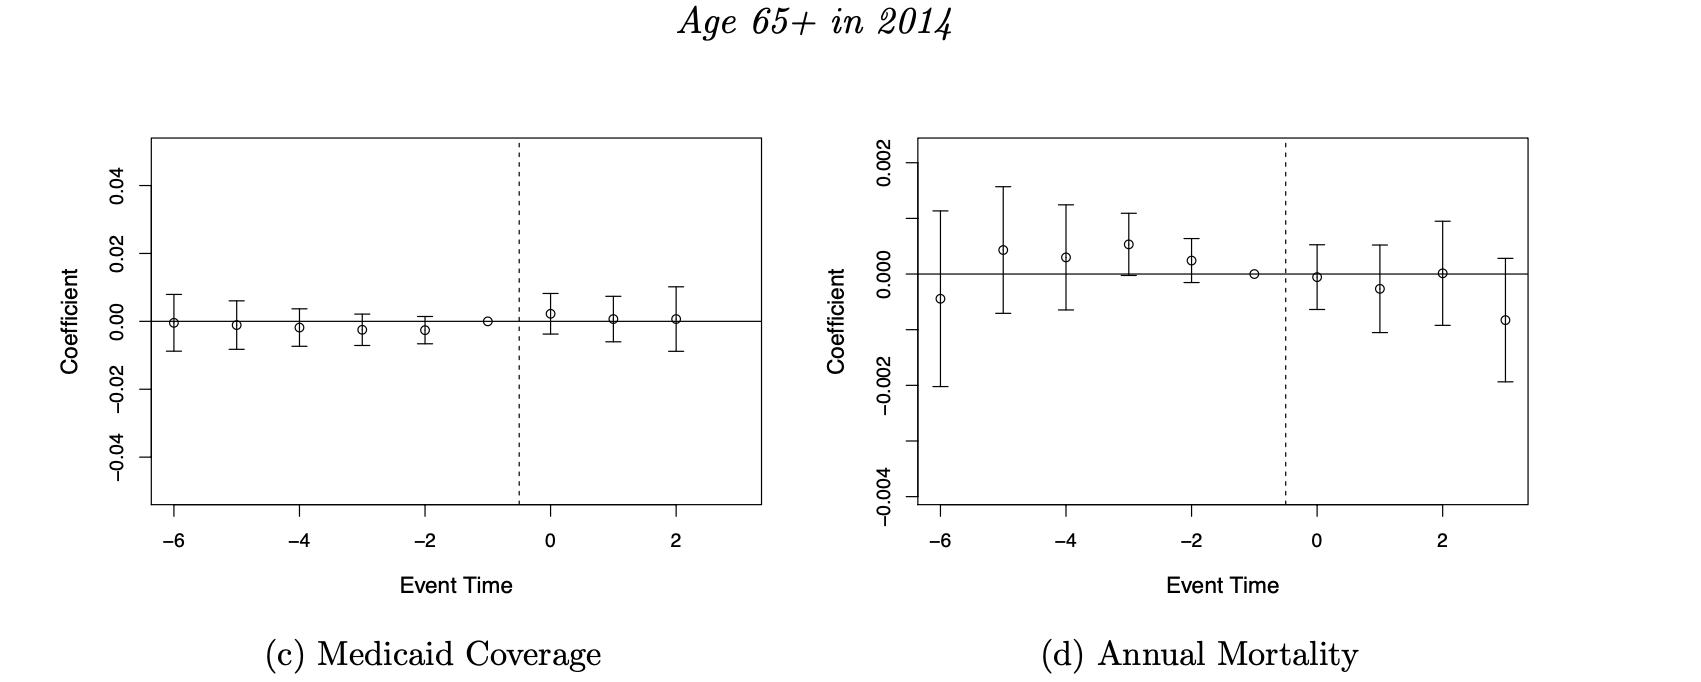
\includegraphics[scale=0.425]{./lecture_includes/placebo_medicaid}
		\end{figure}

\end{frame}

\begin{frame}{Falsification 2: same treatment group, different outcome}

\begin{itemize}
    \item Ask: what else might explain your estimated effect?
    \item Then test whether \emph{that} explanation affects other outcomes your treatment shouldn't.
    \item Example: A policy restricts pseudoephedrine, a key ingredient in meth production.
    \begin{itemize}
        \item Concern: maybe meth production falls not because of the policy, but due to broader drug enforcement efforts.
        \item Falsification: test if violent crimes also fall—if they do, policing may be the real driver.
    \end{itemize}
    \item But be careful: some outcomes (like heroin use) might plausibly change if they’re complements or substitutes.
    \item Goal: use logic, not labels—your falsification should test a story that could undermine your main claim.
\end{itemize}

\end{frame}


\begin{frame}{Rational addiction as a placebo critique}


Sometimes, an empirical literature may be criticized using nothing more than placebo analysis

\begin{quote}``A majority of [our] respondents believe the literature is a success story that demonstrates the power of economic reasoning.  At the same time, they also believe the empirical evidence is weak, and they disagree both on the type of evidence that would validate the theory and the policy implications. Taken together, this points to an interesting gap.  On the one hand, most of the respondents claim that the theory has valuable real world implications.  On the other hand, they do not believe the theory has received empirical support.''
\end{quote}

\end{frame}

\begin{frame}{Placebo as critique of empirical rational addiction}

\begin{itemize}
	\item Auld and Grootendorst (2004) estimated standard ``rational addiction'' models (Becker and Murphy 1988) on data with milk, eggs, oranges and apples.
	\item They find these plausibly non-addictive goods are addictive, which casts doubt on the empirical rational addiction models.
\end{itemize}

\end{frame}

\begin{frame}{Placebo as critique of peer effects}

\begin{itemize}
	\item Several studies found evidence for ``peer effects'' involving inter-peer transmission of smoking, alcohol use and happiness tendencies
	\item Christakis and Fowler (2007) found significant network effects on outcomes like obesity
	\item Cohen-Cole and Fletcher (2008) use similar models and data and find similar network ``effects'' for things that \emph{aren't} contagious like acne, height and headaches
	\item Maybe tall people have tall friends because basketball players are friends with one another?
\end{itemize}

\end{frame}



\subsection{Triple Differences}

\begin{frame}{Triple differences is a research design, not a falsification}

\begin{itemize}

\item Many people equate triple differences with falsification exercise, but it isn't -- it is it's a \emph{design}
\item You use triple differences when you have a parallel trends violation -- that is, when your diff-if-diff is biased
\item Triple differences may sound like a falsification, but it isn't -- it's a research design you use when parallel trends is violated
\item Miller, Johnson and Wherry (2021) didn't use triple differences with near elderly because they didn't think they had a parallel trends violation -- they used a falsification
\end{itemize}

\end{frame}




\begin{frame}{Biased diff-in-diff \#1}

\begin{table}\centering
\scriptsize
		\caption{Biased diff-in-diff \#1: comparing states}
		\begin{center}
		\begin{tabular}{lll|lc}
		\toprule
		\multicolumn{1}{l}{\textbf{States}}&
		\multicolumn{1}{c}{\textbf{Period}}&
		\multicolumn{1}{c}{\textbf{Outcomes}}&
		\multicolumn{1}{c}{$D_1$}&
		\multicolumn{1}{c}{$D_2$}\\
		\midrule
		Experimental states & Before & $Y=NJ$ \\
		& After & $Y=NJ + NJ_t + D$ & $\textcolor{red}{NJ_t}+D$\\
		\midrule
		& & & & $D + (\textcolor{red}{NJ_t}- PA_t)$ \\
		\midrule
		Non-experimental  & Before & $Y=PA$ \\
		states& After & $Y=PA + PA_t$ & $PA_t$\\
		\bottomrule
		\end{tabular}
		\end{center}
	\end{table}

\begin{eqnarray*}
\widehat{\delta}^{true}_{did} = D + (\textcolor{red}{NJ_t} \neq PA_t)
\end{eqnarray*}In other words, you suspect that parallel trends was violated and thus diff-in-diff has no causal interpretation.

\end{frame}


\begin{frame}{Biased Placebo diff-in-diff}

\begin{table}\centering
\scriptsize
		\caption{Biased placebo diff-in-diff: comparing states but single men and older women}
		\begin{center}
		\begin{tabular}{lll|lc}
		\toprule
		\multicolumn{1}{l}{\textbf{States}}&
		\multicolumn{1}{c}{\textbf{Period}}&
		\multicolumn{1}{c}{\textbf{Outcomes}}&
		\multicolumn{1}{c}{$D_1$}&
		\multicolumn{1}{c}{$D_2$}\\
		\midrule
		Experimental states & Before & $Y=NJ$ \\
		& After & $Y=NJ + NJ_t $ & $\textcolor{black}{NJ_t}$\\
		\midrule
		& & & & $ (\textcolor{black}{NJ_t}- PA_t)$ \\
		\midrule
		Non-experimental  & Before & $Y=PA$ \\
		states& After & $Y=PA + PA_t$ & $PA_t$\\
		\bottomrule
		\end{tabular}
		\end{center}
	\end{table}

\begin{eqnarray*}
\widehat{\delta}^{placebo}_{did} = (\textcolor{black}{NJ_t}- PA_t)
\end{eqnarray*}Parallel trends \emph{also} does not hold, $(\textcolor{black}{NJ_t} \neq PA_t)$,

\end{frame}


\begin{frame}{Two biased diff-in-diffs}

\begin{itemize}


\item Parallel trends does not hold, $(\textcolor{red}{NJ_t} \neq PA_t)$, but what if that's the same bias in our placebo DiD?
\item Then we can subtract the placebo diff-in-diff from the "true diff-in-diff": $$ \widehat{\delta}_{ddd} = \widehat{\delta}^{true}_{did} - \widehat{\delta}^{placebo}_{did}$$
\item Triple differences is a ``real design'' with one parallel trends assumption: $$(\textcolor{red}{NJ_t}^{true}- PA_t^{true}) = (\textcolor{black}{NJ_t}^{placebo}- PA_t^{placebo})$$

\end{itemize}

\end{frame}

\begin{frame}{Triple differences by Gruber (1995)}

	\begin{figure}
	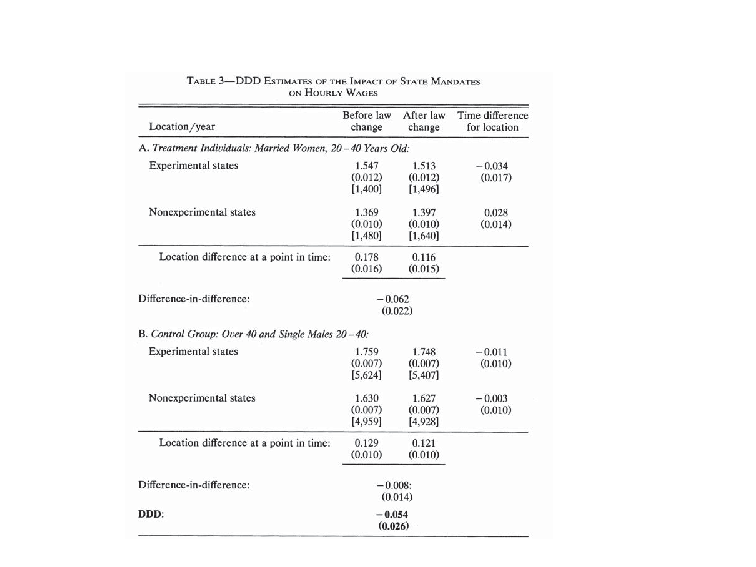
\includegraphics{./lecture_includes/gruber_ddd_3.pdf}
	\end{figure}

\end{frame}

\begin{frame}{Triple differences commentary}

\begin{itemize}
\item Some people think that it requires that the placebo DiD be zero, but that's incorrect

\item In Gruber's 1995 article, it isn't clear why he needed triple differences in the first place -- his triple differences yielded -0.054 which is almost the same as what he found with his first diff-in-diff (-0.062)
\item The main value of triple differences is that you use it when you believe the parallel trends assumption doesn't hold

\end{itemize}

\end{frame}


\begin{frame}[shrink=20]

\begin{table}\centering
		\caption{Difference-in-Difference-in-Differences (Gruber version)}
		\tiny
		\begin{center}
		\begin{tabular}{lll|l|lll}
		\toprule
		\multicolumn{1}{l}{\textbf{Groups}}&
		\multicolumn{1}{c}{\textbf{States}}&
		\multicolumn{1}{c}{\textbf{Period}}&
		\multicolumn{1}{c}{\textbf{Outcomes}}&
		\multicolumn{1}{c}{$D_1$}&
		\multicolumn{1}{c}{$D_2$}&
		\multicolumn{1}{c}{$D_3$}\\
		\midrule
		&&After	&$NJ+MW+\textcolor{blue}{NJ_t}+\textcolor{red}{MW_t}+D$					\\
	&Experimental			&&&$\textcolor{blue}{NJ_t}+MW_t + D$			\\
		&states&Before	&$NJ+MW$					\\
Married women 					&&&&&$D+\textcolor{blue}{NJ_t} -PA_t 	$	\\
20-40							&&&&&$$\\
    		&&After	&$PA+MW+PA_t+MW_t$					\\
	&Non-experimental		&&	&$PA_t+MW_t$				\\
		&states&Before	&$PA+MW$					\\
								\\
&&&&&&$\textcolor{black}{D}$
\\
		&&After	&$NJ+SO+NJ_t+SO_t$				\\
	&Experimental 			&&&$NJ_t+SO_t$ \\
		&states&Before	&$NJ+SO$					\\
Single men 					&&&&&$NJ_t  - PA_t$		\\
Older women					&&&&&$$		\\
	     	&&After	&$PA+SO+PA_t+SO_t$					\\
	&Non-experimental		&&&	$PA_t+SO_t$				\\
		&states&Before	&$PA+SO$					\\
		\bottomrule
		\end{tabular}
		\end{center}
	\end{table}

\begin{center}
\textbf{Triple diff assumption}
\end{center}

$\widehat{\delta}_{DDD}= D + \underbrace{[(\textcolor{blue}{NJ^{MW}_t} - PA^{MW}_t) -( NJ^{SO}_t - PA^{SO}_t )]}_{\mathclap{\text{Equally biased  DiD \#1 and \# 2}}}$

\bigskip
Triple differences requires two diff-in-diff, from different groups, with the same bias. Parallel bias


\end{frame}







\begin{frame}{DDD in Regression}

	\begin{eqnarray*}
	Y_{ijt} &=&\alpha +  \beta_2 \tau_t + \beta_3 \delta_j  + \beta_4 D_i + \beta_5(\delta \times \tau)_{jt} \\
	&& +\ \beta_6(\tau \times D)_{ti} +  \beta_7(\delta \times D)_{ij} +  \textcolor{red}{\beta_8(\delta \times \tau \times  D)_{ijt}}+  \varepsilon_{ijt}
	\end{eqnarray*}

	\begin{itemize}
	\item Your dataset will be stacked by group $j$ and state $i$
	\item $\widehat{\beta_8}$ estimates the ATT
	\item Parallel bias, NA and SUTVA necessary and sufficient for identification
	\end{itemize}

\end{frame}



\begin{frame}{Simulation}

In /Labs/DDD I have a simulation to illustrate this for us called ddd2.do.  The ATT is -\$5,000 but the biased DiD is -\$7487.  The non-parallel trends bias is -\$2,487.  So I replicate Gruber (with simulated data) where the placebo DiD is close (-\$2,507).  I then present a triple differences which gives us -\$4,972. Let's look at the final product.

\end{frame}

\begin{frame}{Triple differences event study}

\begin{figure}
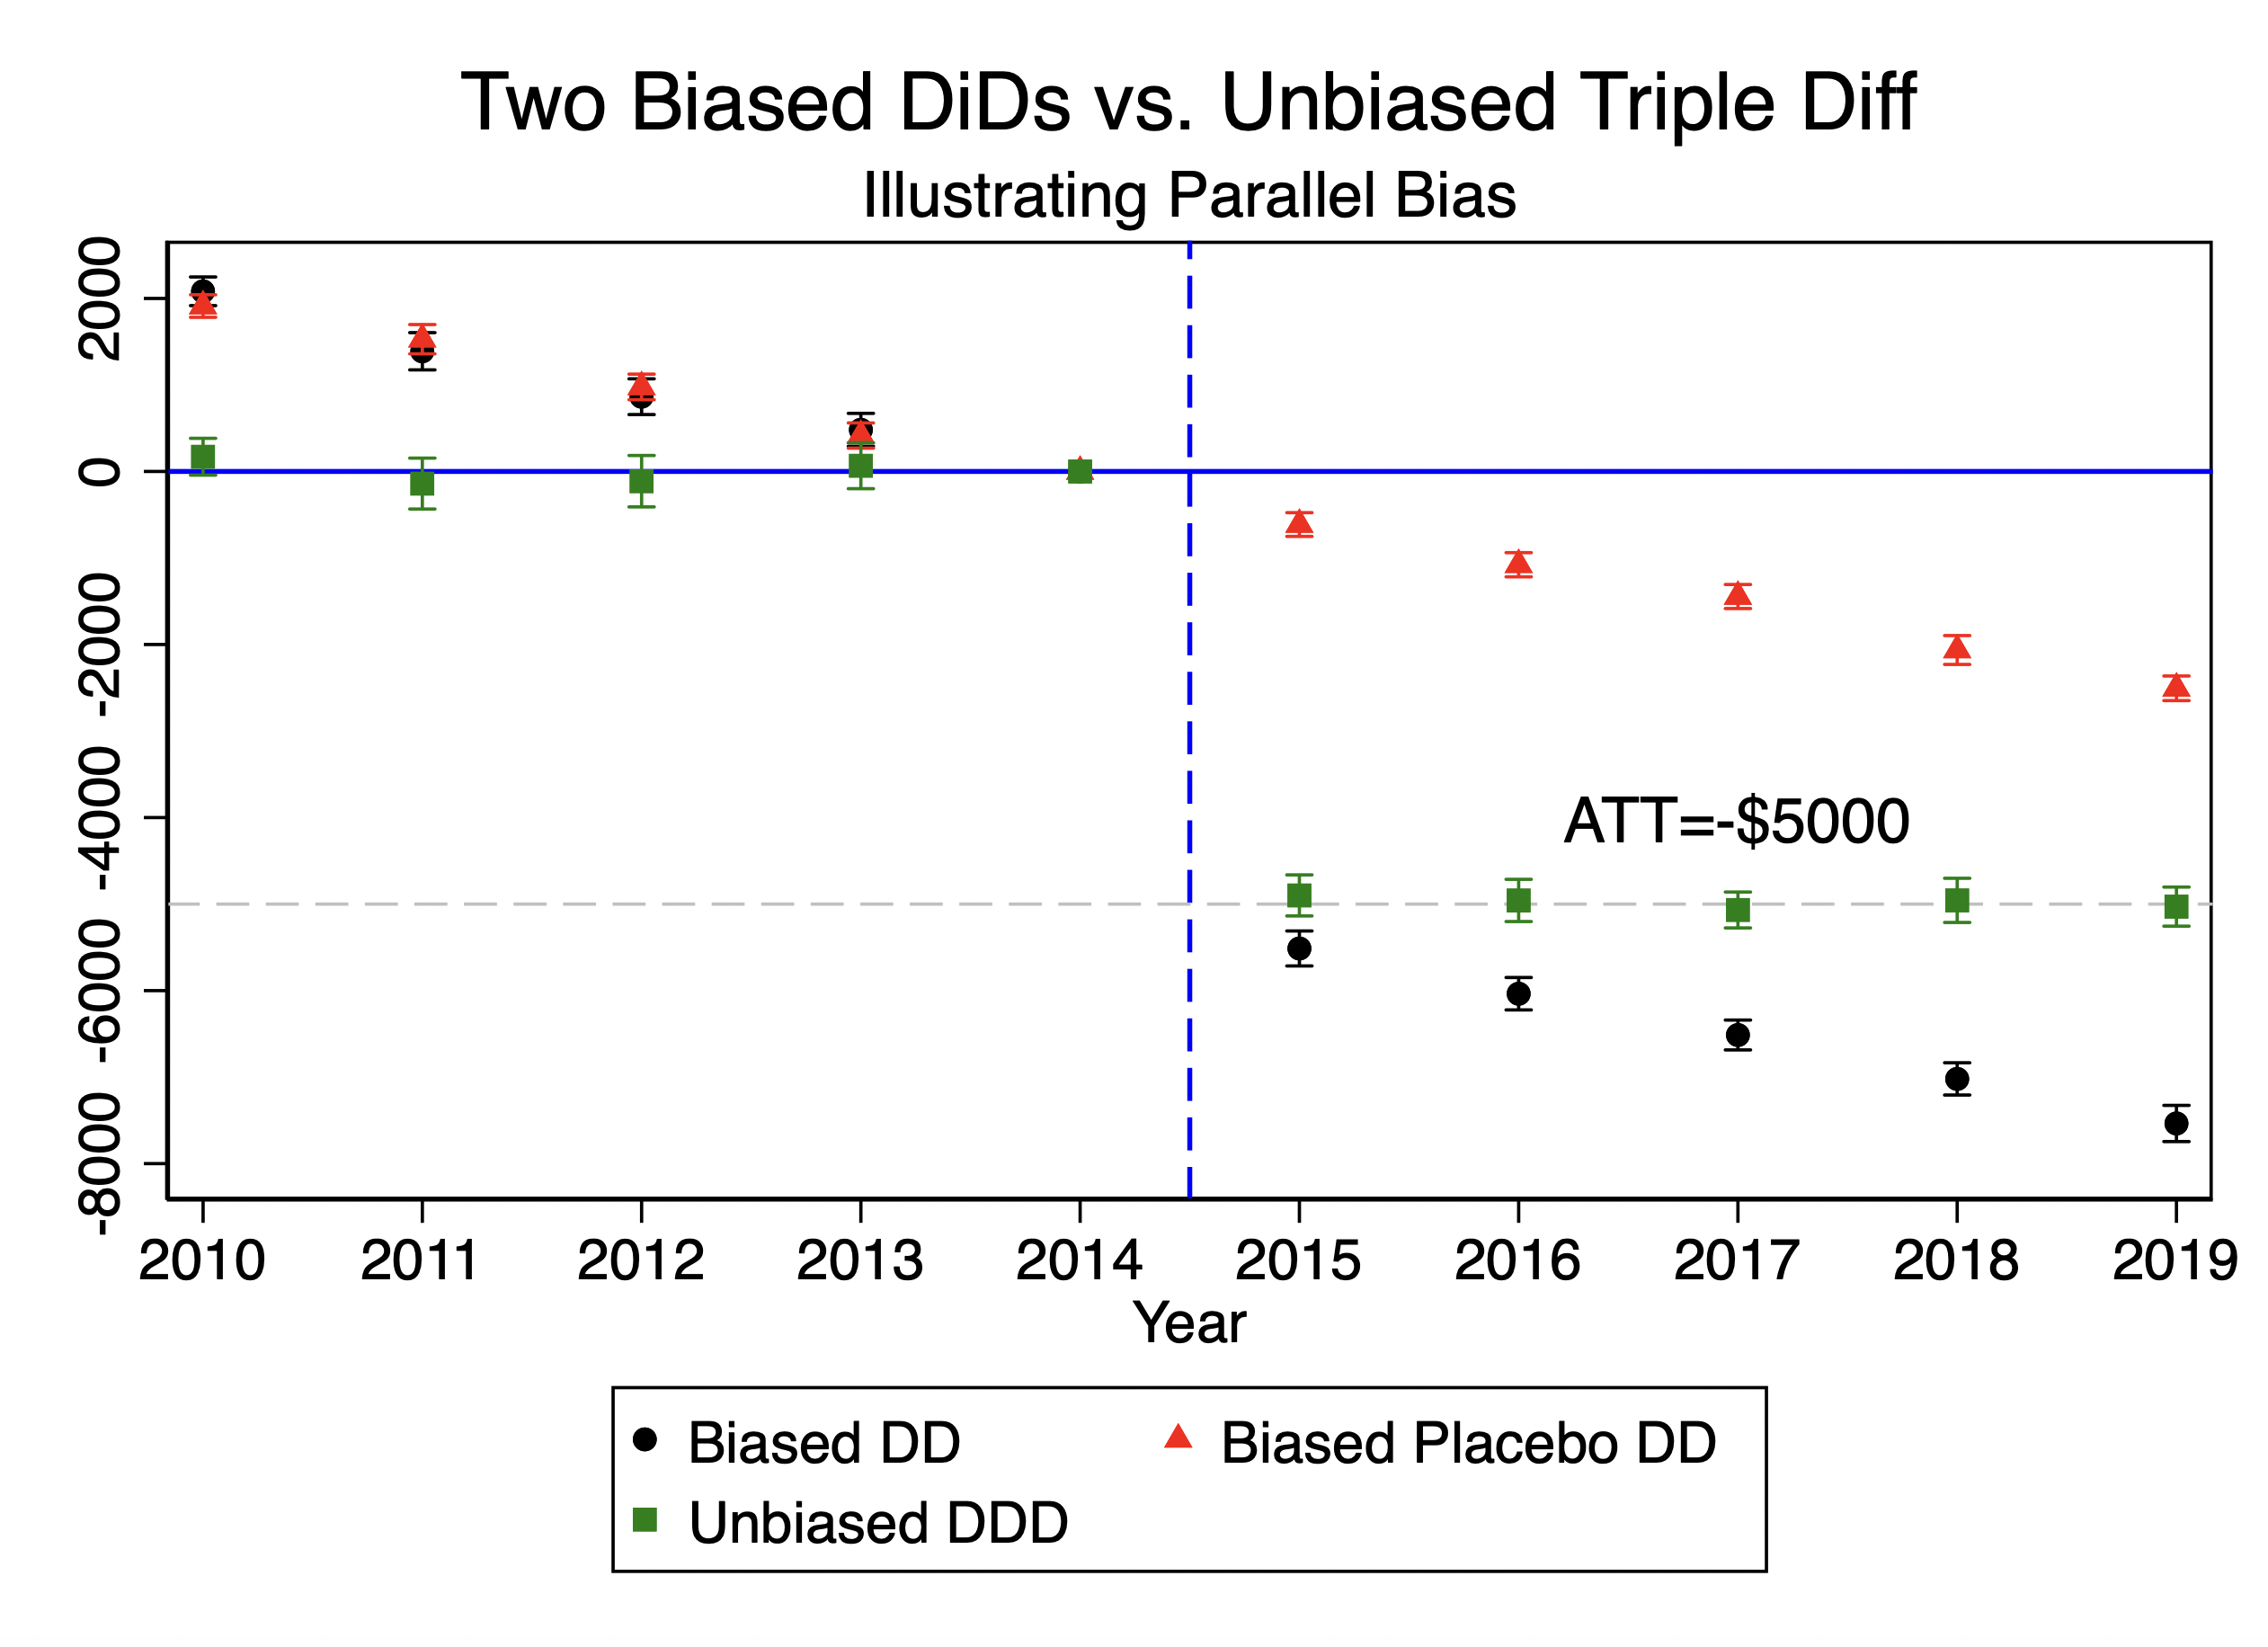
\includegraphics[scale=0.25]{./lecture_includes/ddd_simulation}
\end{figure}



\end{frame}

\begin{frame}{Great new paper to learn more}

\begin{figure}

\includegraphics[scale=0.25]{./lecture_includes/olden_moen_2022_ddd.png}
\end{figure}

\end{frame}


\begin{frame}{Summarizing DDD}

\begin{itemize}
\item Used to be people thought DDD required two parallel trends assumptions but it does not -- it is a real design and requires one parallel trends assumption
\item Parallel trends assumption is ``parallel bias'' -- that the bias of the true DiD is the same as the bias of the placebo DiD
\item The ladder of evidence still holds -- you'll want to present the event study plot, and my code provides it for you, because you need to evaluate the parallel bias assumption
\item Given the lack of triple diff literacy, you may have to write this anticipating reader and maybe editor confusion and so "educate" as you go -- overlaying all three plots could be help

\end{itemize}

\end{frame}




\section{Covariates}

\subsection{Compositional Change}

\begin{frame}{Repeated cross-sections and compositional change}

	\begin{itemize}
	\item One of the risks of a repeated cross-section is that the composition of the sample may have changed between the pre and post period in ways that are correlated with treatment
	\item Hong (2013) uses repeated cross-sectional data from the Consumer Expenditure Survey (CEX) containing music expenditure and internet use for a random sample of households
	\item Study exploits the emergence of Napster (first file sharing software widely used by Internet users) in June 1999 as a natural experiment
	\item Study compares internet users and internet non-users before and after emergence of Napster
	\end{itemize}

\end{frame}

\begin{frame}{Introduction of Napster and spending on music}
	\begin{figure}
	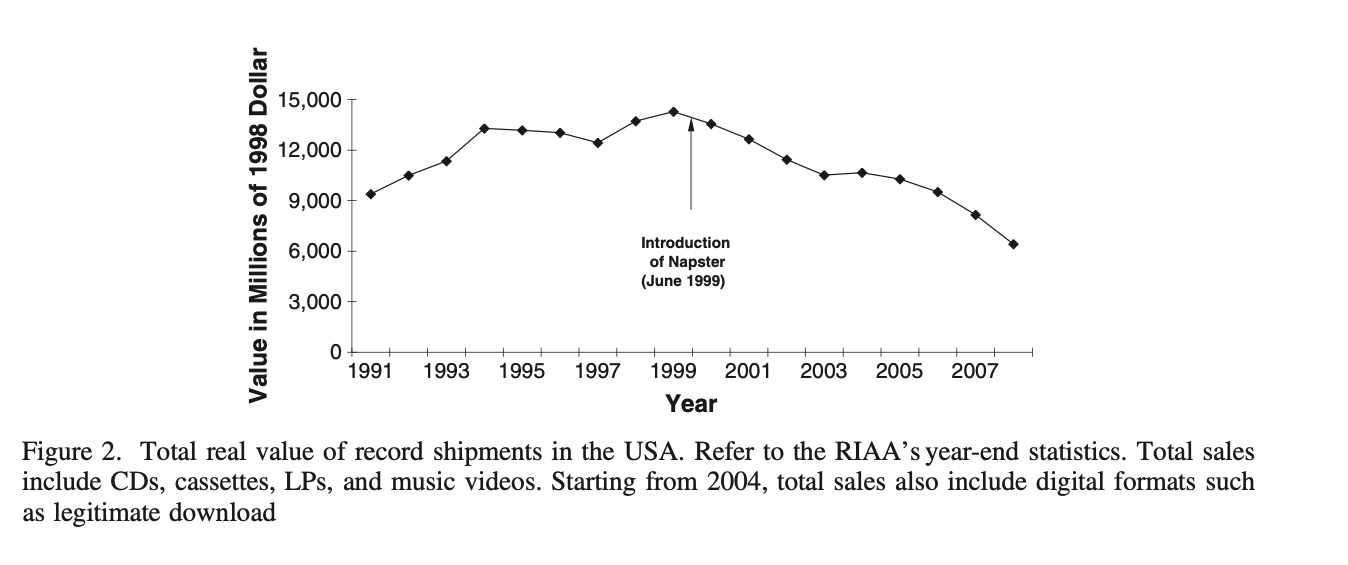
\includegraphics[scale=0.5]{./lecture_includes/hong_napster}
	\end{figure}

\end{frame}


\begin{frame}[plain]
	\begin{figure}
	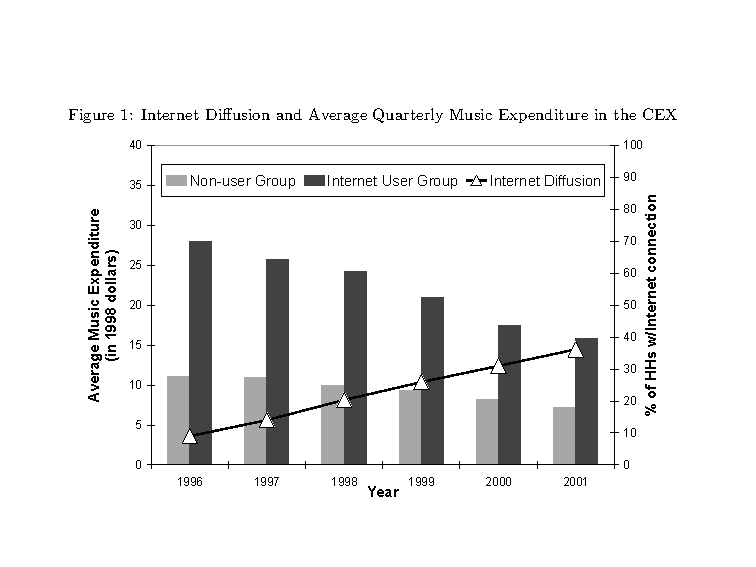
\includegraphics{./lecture_includes/Hong_1.pdf}
	\end{figure}

\end{frame}



\begin{frame}{Repeated Cross Section Risks}

\begin{itemize}
\item Repeated cross sections have their own challenges that panels don't in that the group could be shifting compositionally
\item Detect using a balance table with covariates highly predictive of the missing $E[Y^0|D=1]$ for this exercise
	\begin{itemize}
	\item Percent of cat owners is probably irrelevant to trends in potential outcomes
	\item But age and income is probably relevant for spending habits
	\item We'll discuss covariates more later, but for now just consider what characteristics are relevant to your outcome
	\end{itemize}
\item Documenting covariates that are cannot be affected by the treatment like this table is a way to check for \emph{compositional changes} in the sample
\end{itemize}

\end{frame}


\begin{frame}{Changes Between Internet and Non-Internet Users Over Time}

	\begin{figure}
	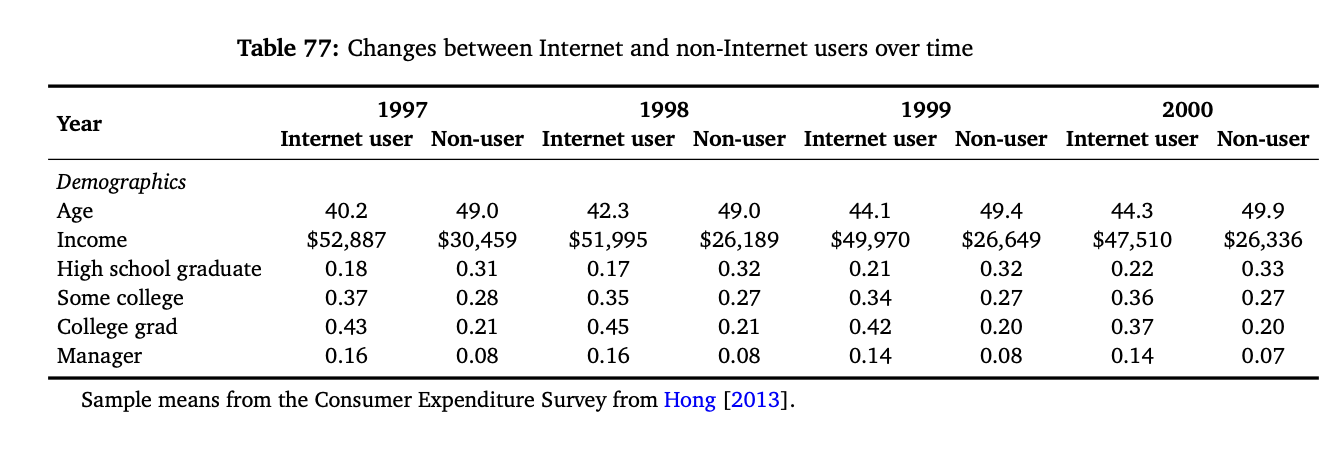
\includegraphics[scale=0.5]{./lecture_includes/hong_table.png}
	\end{figure}



\end{frame}



\begin{frame}{What was this table about?}

\begin{itemize}
\item  Notice that users are getting older and poorer -- both of which predict spending less money on music
\item If these covariates are themselves predictive of trends, then it is suggestive parallel trends could be \emph{mechanically} breaking, so estimate $$X_{it} = \alpha + \beta_1 D_i + \beta_t Post_t + \delta ( D_i \times Post_t ) + \varepsilon_{it}$$
\item Or consider the normalized difference in means table we discuss later
\item If violated, then consider the following fix by Hong (2013) which adjusts for propensity scores in both periods
\end{itemize}

\end{frame}



\begin{frame}{Step 1. Estimate Propensity Scores}
\begin{itemize}
  \item Estimate two separate propensity scores -- one for each time period
  \item Pre-treatment period ($T = 0$) uses both treated and control units (as $Y=Y^0$ for both)
  \begin{equation*}
    P_b = \Pr(D=1 \mid T=0, X)
  \end{equation*}
  \item Post-treatment period ($T = 1$) using only control group units (as $Y=Y^0$ for control only)
  \begin{equation*}
    P_a = \Pr(D=1 \mid T=1, X)
  \end{equation*}
\end{itemize}
\end{frame}

\begin{frame}{Step 2. Weight Observations Using Propensity Scores}
\begin{itemize}
  \item Use inverse probability weighting (IPW) to balance samples:
    \item For the pre-treatment period (\( T = 0 \)):
  \begin{align*}
        E_w[Y \mid D = 1, T = 0] &= \frac{\sum_{i \in T=0, D=1} Y_i / P_b(X_i)}{\sum_{i \in T=0, D=1} 1 / P_b(X_i)} \\
        E_w[Y \mid D = 0, T = 0] &= \frac{\sum_{i \in T=0, D=0} Y_i / (1 - P_b(X_i))}{\sum_{i \in T=0, D=0} 1 / (1 - P_b(X_i))}
  \end{align*}
    \item For the post-treatment period (\( T = 1 \)):
  \begin{align*}
        E_w[Y \mid D = 1, T = 1] &= \frac{\sum_{i \in T=1, D=1} Y_i / P_a(X_i)}{\sum_{i \in T=1, D=1} 1 / P_a(X_i)} \\
        E_w[Y \mid D = 0, T = 1] &= \frac{\sum_{i \in T=1, D=0} Y_i / (1 - P_a(X_i))}{\sum_{i \in T=1, D=0} 1 / (1 - P_a(X_i))}
  \end{align*}
\end{itemize}
\end{frame}

\begin{frame}{Step 3. Calculate the Adjusted Difference-in-Differences}
\begin{itemize}
  \item Use the weighted averages to compute the adjusted DiD estimator:
  \begin{align*}
    \text{Adjusted DiD} &= \left( E_w[Y \mid D = 1, T = 1] - E_w[Y \mid D = 0, T = 1] \right) \nonumber \\
    &\quad - \left( E_w[Y \mid D = 1, T = 0] - E_w[Y \mid D = 0, T = 0] \right)
  \end{align*}
  \item This accounts for compositional change and enhances credibility of ATT estimation in repeated cross-sections.
\end{itemize}
\end{frame}


\begin{frame}{Reweighted regressions}

\begin{itemize}
\item It's a reweighted 2x2 estimator which we know how as an OLS equivalence
\item You're going to use as analytical weights the IPW formulas and one of the regressions with WLS
\item But make sure you are using \emph{both} IPW expressions -- it is two propensity score formulas, not one
\end{itemize}

\end{frame}

\begin{frame}{Value of the method}

\begin{itemize}
\item Panel datasets are expensive because following the same people over time is expensive
	\begin{itemize}
	\item Tracking respondents, maintaining contact, managing attrition
	\item Many countries, particularly in the Global South, have fewer of them than in highly developed countries
	\end{itemize}
\item Repeated cross sections are often more common -- rich, nationally representative datasets collected in waves, but with different individuals each time
\item Hong's estimator was developed precisely for this context -- an estimator that can account for the changing compositional changes (a problem that happens often, but is rarely addressed)
\item Diagnostic tools are also very intuitive -- balance tables, seemingly unrelated regressions on multiple covariates

\end{itemize}

\end{frame}






\subsection{Conditional Parallel Trends}

\begin{frame}{Is Unconditional Parallel Trends Plausible?}

\begin{itemize}

\item We have been working with a parallel trends assumption that requires the two \emph{groups} have the same trend in average $Y^0$

\item But what if these two groups were so different from one another that their potential outcomes didn't add up to be the same?

\item What if the workers in the job training program were poor and the control group was rich -- do we think the earnings of those two groups would have been evolved similarly?  Why/why not?



\end{itemize}

\end{frame}


\begin{frame}{You may need a \emph{different} PT assumption}

\begin{itemize}
\item Parallel trends for sub-populations, but not the whole population:
	\begin{enumerate}
	\item Unconditional parallel trends:  parallel trends holds for the overall average treatment and control groups
	\item Conditional parallel trends: parallel trends only has to hold for observable sub-groups, but not necessarily the whole group
	\end{enumerate}
\item Example: Male versus female earnings growth
	\begin{itemize}
	\item Assume male earnings grow by $+2$, female by $+1$,
	\item Treatment is 75\% male, control is 25\% is male
	\item $E[\Delta Y^0|D=1]=1.75$ but $E[\Delta Y^0|D=0]=1.25$
	\end{itemize}
\item Unconditional parallel trends won't hold because the groups aren't balanced on the characteristics that cause trends
\end{itemize}

\end{frame}



\begin{frame}{Conditional parallel trends}
Conditional parallel trends (CPT) is a weakened version of the parallel trends assumption requiring that it holds \emph{within} the dimensions of the selected covariates:
\begin{align*}
CPT: \textcolor{red}{E[Y^0_k|Post, X]} - E[Y^0_k|Pre, X] = E[Y^0_U|Post, X] - E[Y^0_U|Pre, X]
\end{align*}
First time it shows up is Heckman, Ichimura and Todd (1997). Idea can be abstract so let's look at a graph to help us decipher what it means and what we can do. And it's still not directly testable due to still missing the first potential outcome (i.e., counterfactual).
\end{frame}

\begin{frame}{Which covariates do you need?}

\begin{itemize}
\item Conditional parallel trends is tricky because it first assumes you know the covariates you need to satisfy it
\item But how do we decide which variables do this and which ones don't?
\item Econometrics is no help here -- you need common sense, theory, logic, and expertise
\item When selecting covariates, use "confounders" logic -- but confounders of the \emph{trend}?
\end{itemize}

\end{frame}




\begin{frame}{Graphs Can Help Pick Covariates}

\begin{figure}[h!]
    \centering
    \begin{tikzpicture}[
        node distance=2.5cm,
        every node/.style={align=center},
        line/.style={->, thick},
    ]
    % Nodes
    \node (X) {Covariates \\ \( X \)};
    \node (D) [below left of=X, xshift=-1cm, yshift=-1cm] {\( D \)};
    \node (DeltaY0) [below right of=X, xshift=1cm, yshift=-1cm] {\( \Delta E\left[Y^0\right] \)};
    % Arrows
    \draw[line] (X) -- (DeltaY0);
    \draw[line] (X) -- (D);
    \end{tikzpicture}
\caption{DAG representing differences in county-level covariate composition (\(X\)) across treatment and control groups (\(D\)) and their determination of the untreated potential outcome trends (\(\Delta E\left[Y^0\right]\)).}
\end{figure}

\end{frame}



\begin{frame}{Example: Concealed Carry Gun Laws and Murder}

\begin{itemize}
\item Become an expert on your left-hand-side variable because you need to know $X \rightarrow \Delta Y^0$
	\begin{itemize}
	\item Drugs and gangs (i.e., crack cocaine epidemic)
	\item Cities had different homicide rates than rural counties
	\item Police, incarceration
	\item Demographics (e.g., race shares, age shares) and economic things (e.g., poverty, per capital income, AFDC rolls)
	\item Consider LASSO in the pre-periods only to select covariates predictive of pre-treatment \emph{untreated potential outcome} trends (i.e., $\Delta Y^0$)
	\end{itemize}
\end{itemize}

\end{frame}




\begin{frame}{Covariate Imbalance}
    \begin{itemize}
	\item Kahn-Lang and Lang (2020) say that if your two groups are different at baseline on outcomes, treatment was not random, is likely caused by covariates, and you need to explain why that matters or does not
	\item Randomized treatment will balance covariates, hence why we don't need to include them as controls in RCT \emph{even though they cause the outcome}
	\item But if they aren't balanced in your diff-in-diff, and they cause \emph{trends}, then parallel trends won't hold
\item So, next you focus on $X \rightarrow D$, which is to say, check the imbalance in covariates you need for conditional parallel trends
\end{itemize}
\end{frame}



\begin{frame}{Create a balance table}

\begin{figure}
    \centering
    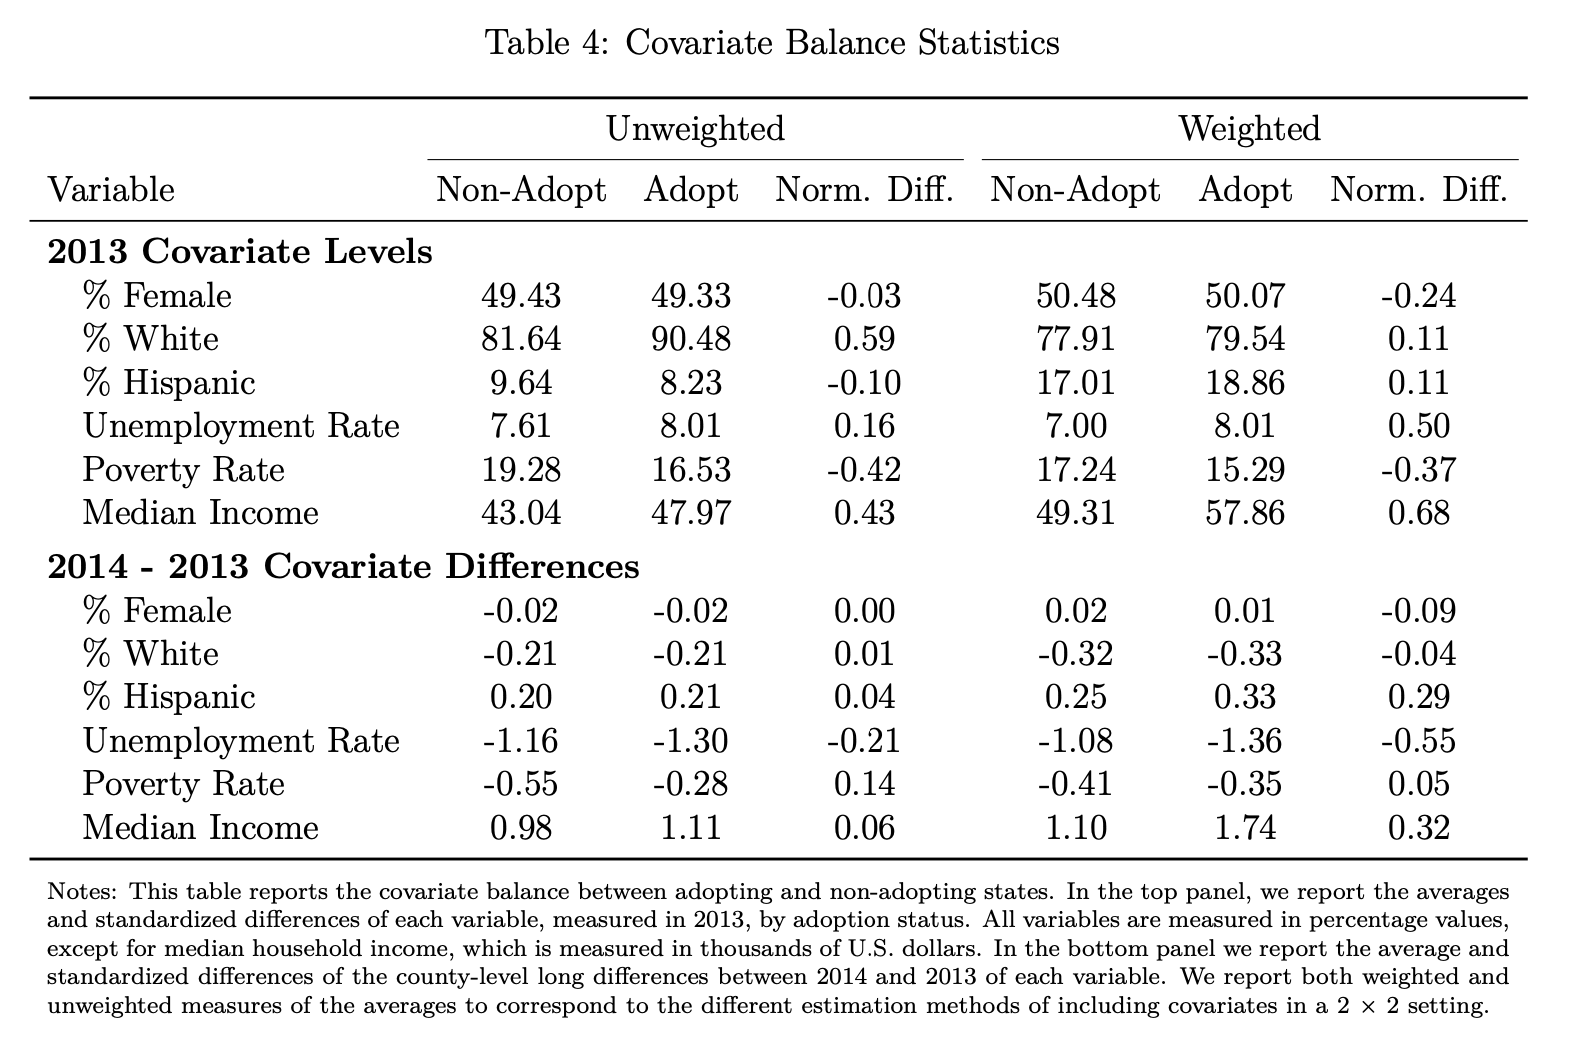
\includegraphics[height=0.80\textheight]{./lecture_includes/step6_imbalance}
\end{figure}

\end{frame}


\begin{frame}
    \frametitle{Baseline Covariates and Normalized Difference}
    \begin{itemize}
        \item Baseline covariates are measured before treatment ($t-1$).
        \item Report the averages of covariates for both groups in a table and the "normalized difference in means" calculated as:
        $$ \text{Norm. Diff}_\omega = \frac{\overline{X}_{\omega,T} - \overline{X}_{\omega,C}}{\sqrt{(S_{\omega,T}^2 + S_{\omega,C}^2)/2}} $$
        \item The normalized difference measures imbalance; it should be less than 0.25 in absolute value to avoid problematic imbalance (Imbens and Rubin 2015).
    \end{itemize}
\end{frame}


\begin{frame}
    \frametitle{Summarizing}
    \begin{itemize}
    \item So, when choosing covariates, remember that there are two steps involved
    	\begin{enumerate}
	\item $X \rightarrow \Delta E[Y^0]$. Pick covariates that are needed to satisfying conditional parallel trends
	\item $X \rightarrow D$. Check for imbalance using the normalized difference in means equation to determine if you have "problematic imbalance"
	\end{enumerate}
\item And the heuristic I am suggesting is to select covariates that are the "ordinary determinants of $Y^0$" (i.e., become an expert on your left-hand-side variable)
    \end{itemize}
\end{frame}






\subsection{Four Estimators for Covariates}

\begin{frame}{Estimators for Covariates}

\begin{itemize}

\item But, let's say that we feel we have to assume conditional parallel trends
\item What estimators can accomodate that assumption with the least amount of assumptions?
\item We will review four now:
	\begin{enumerate}
	\item Inverse probability weighting
	\item Outcome regression
	\item Double robust
	\item Regressions
	\end{enumerate}
\end{itemize}

\end{frame}


\begin{frame}{Three key covariate estimators in diff-in-diff}

Three papers (though sometimes you see others) about covariate adjustment in DiD:
\begin{enumerate}
\item Abadie (2005) on semiparametric DiD -- reweights the comparison group part of the DID equation using a propensity score based on X
\item Heckman, Ichimura and Todd (1997) on outcome regression uses baseline X and control group only to impute the missing counterfactual $Y^0$ for treatment group units in a DiD equation
\item Sant'Anna and Zhao (2020) is double robust which means the method does both of these at the same time so that you don't have to choose between them
\end{enumerate}

\bigskip

We will discuss both of them and then compare their performance with the more straightforward fixed effects model

\end{frame}






\begin{frame}{Inverse probability weighting}


 Abadie (2005) proposed a model that simply reweights the control group in the DiD equation using a particular specification (``semiparametric'') of the propensity score on pretreatment covariates

	\begin{enumerate}
	\item Calculate each unit's ``after minus before'' (DiD equation)
	\item Estimate the conditional probability of treatment based on baseline covariates (propensity score estimation)
	\item Weight the comparison group's DiD equation with the propensity score
	\end{enumerate}

Remember -- ATT is only missing $Y^0$ for treatment, so we only have to apply weights to the comparison group units

\end{frame}

\begin{frame}{Novel elements of time in Abadie's model}

\begin{itemize}
\item There is only one treatment group so therefore there is only one relevant treatment date, $t$
\item The period prior to treatment is called the baseline, or $b$, period and it is when treated units were not treated
\item $X_b$ are ``baseline'' covariates meaning the value of $X$ in the pre-treatment period for either the treated or comparison group units
\item Propensity scores are estimated off the $b$ period \emph{only}
\item Abadie ``throws away'' covariates after treatment because this is all about re-establishing parallel trends which is a \emph{baseline} concept recall
\end{itemize}

\end{frame}

\begin{frame}{Assumptions}

Four main assumptions

\begin{enumerate}
\item No anticipation
\item Conditional parallel trends $$E[Y^0_t - Y^0_b|D=1,X_b] = E[Y^0_t - Y^0_b | D=0, X_b]$$
\item Common support $$Pr(D=1)>0; Pr(D=1|X)<1$$
\item Propensity score model is properly specified
\end{enumerate}

\end{frame}

\begin{frame}{Propensity scores as dimension reduction}

\begin{itemize}

\item Propensity scores are ways of dealing with a conditioning set $X$ that has large dimensions
\item Dimensions are not the same as covariates -- if you have continuous $X$, then it has infinite dimensions
\item Common support means that \emph{within} all combinations of the covariates (e.g., white male 47yo versus whites, males, age) there are units in treatment and control

\end{itemize}

\end{frame}

\begin{frame}{Common support example}

Think of common support like ``exact matches'' but on the propensity score

\bigskip

I'm a white male 47 years old with a PhD; can I find a white male 47 years old without a PhD

\bigskip

If I can, that's common support; if I cannot that's off support

\end{frame}


\begin{frame}{Propensity scores as dimension reduction}

\begin{itemize}

\item Propensity score theorem (Rosenbaum and Rubin 1983) showed that if you need $X$ to satisfy some assumption, the propensity score will satisfy too
\item Propensity scores essentially transform your large dimensional problem into a single scalar called the propensity score, which is the conditional probability of treatment (conditional on $X$)
\item But we need to estimate the propensity score because we don't usually know it (only an experimentalist ``knows'' the true propensity score)

\end{itemize}

\end{frame}

\begin{frame}{Common support and the propensity score}

\begin{itemize}
\item Exact matches mean you have people who are identical on covariate values in both treatment and control
\item Common support and the propensity score means you have people nearly identical on their probability of treatment
\item I am 47yo white male with a PhD with a propensity score of 0.75, but you are an Asian female 27yo without a PhD and have a propensity score of 0.75
\item Same idea, but for this to work, we need to have ``matches'' like that (just on the propensity score)
\end{itemize}

\end{frame}


\begin{frame}{How do these work together?}

Since we are identifying the ATT, and the ATT is missing $Y^0$ for the treated group, we are using the control group $Y^0$ in its place

\bigskip

Under conditional parallel trends and common support, some of the comparison group units are recovering the parallel trends because of their $X$ values creating projections that in their differences perfectly aligned in expectation with the missing $\Delta E[Y^0|D=1]$

\bigskip

But we have to have all three for it to work

\end{frame}

\begin{frame}{Checking for overlap}

\begin{enumerate}
\item Estimate the propensity scores yourself and then plot with histograms to check for overlap
\item Check that the control group propensity scores are not above 0.995 and if so trim them
\end{enumerate}

\end{frame}

\begin{frame}{Checking propensity scores for overlap}

	\begin{figure}
	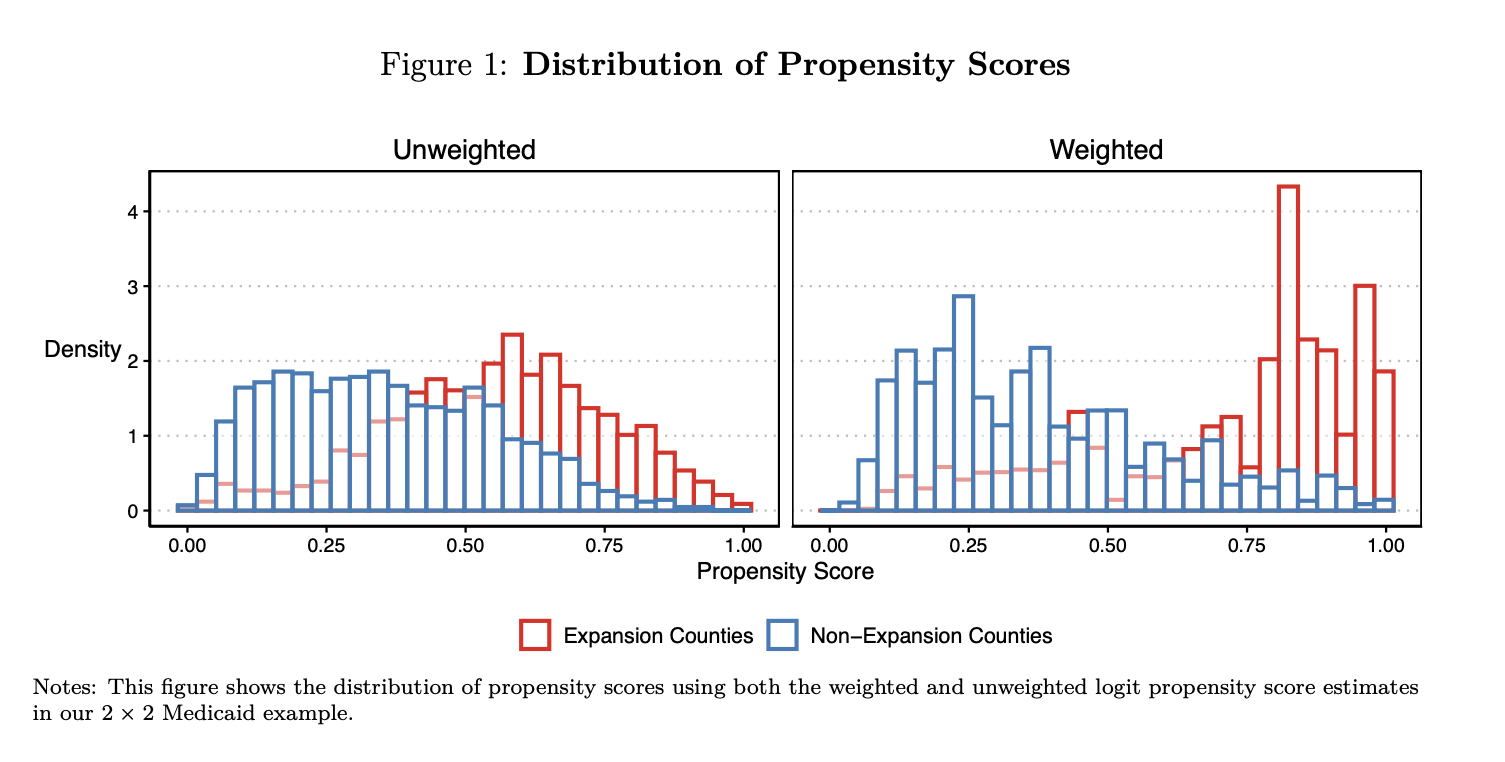
\includegraphics[scale=0.05]{./lecture_includes/baker_pscore.png}
	\end{figure}

\end{frame}

\begin{frame}{Checking for large propensity scores}

\begin{itemize}
\item Abadie's estimator uses the \emph{inverse probability weight} $$\frac{-p(x)}{1-p(x)}$$
\item Consider these examples
	\begin{enumerate}
	\item Control group has $p(x)=0.75$, \emph{IPW} is $\frac{-0.75}{0.25}=-3$. 
	\item Control group has $p(x)=0.25$, \emph{IPW} is $\frac{-0.25}{0.75}=-0.33$
	\end{enumerate}
\item But what if the control group propensity score is almost 1?
	\begin{enumerate}
	\item Control group has $p(x)=0.998$, \emph{IPW} = $\frac{-0.998}{0.002}=-499$
	\end{enumerate}
\item IPW "outliers" are with respect to control group "extremely high propensity scores" -- causes the weights to explode, so trim them
\end{itemize}

\end{frame}


\begin{frame}{Definition and estimation}

Defining the ATT parameter of interest
\begin{eqnarray*}
ATT &=& E[Y^1_t - \textcolor{red}{Y^0_t} |D=1] \\
&=&E[Y^1_t  | D = 1 ] - \textcolor{red}{E[Y^0_t | D=1]}
\end{eqnarray*}

\bigskip
Abadie's inverse probability weighting (IPW) estimator
\begin{eqnarray*}
E\bigg [ \frac{Y_t - Y_b}{Pr(D=1)} \times \frac{D - Pr(D=1|X_b)}{1-Pr(D=1|X_b)} \bigg ]
\end{eqnarray*}

\bigskip

The first is our causal parameter; the second is our reweighted DiD equation that \emph{estimates} our causal parameter, but we need to estimate that propensity score


\end{frame}

\begin{frame}{Abadie's IPW estimator}

Look closely; what happens mathematically when you substitute $D=1$ vs $D=0$?

\begin{eqnarray*}
E\bigg [ \frac{Y_t - Y_b}{Pr(D_t=1)} \times \frac{D_t - Pr(D=1|X_b)}{1-Pr(D=1|X_b)} \bigg ]
\end{eqnarray*}

\bigskip

The reweighting with the propensity only happens to the comparison group's first differences -- not the treatment groups!  Why?  Because it's the $Y^0$ that is missing, not the $Y^1$

\end{frame}



\begin{frame}{Propensity scores}

\begin{itemize}
\item It's common to hear people say that we don't know the propensity score; we can only estimate it. Same here -- we approximate it with regressions
\item Paper is titled ``Semi-parametric DiD'' because Abadie imposes structure on the polynomials used to construct the propensity score (``series logit'')
\end{itemize}

\end{frame}







\begin{frame}{Outcome regression }

\begin{itemize}
\item Outcome regression (OR) models are explicit \emph{imputation} estimators
\item If conditional parallel trends holds, then whatever the relationship is between $X$ and $Y$ for the control group is the same for treatment group
\item You use this idea to fit a model from the control group then impute for the treatment group
\item Core model is Heckman, Ichimura and Todd (1997), RESTUD
\end{itemize}

\end{frame}





\begin{frame}{Identification assumptions I: Conditional parallel trends}

Assumption 1: Conditional parallel trends

\bigskip

Counterfactual trends for the treatment group are the same as the control group for all values of $X$

\begin{eqnarray*}
E[Y_1^0 - Y_0^0 | X, D=1] = E[Y^0_1 - Y^0_0 | X, D=0]
\end{eqnarray*}

\end{frame}

\begin{frame}{Identification assumptions II: Common support}

Assumption 2: Common support

\bigskip

For some $e>0$, the probability of being in the treatment group is greater than $e$ and the probability of being in the treatment group conditional on $X$ is $\leq1-e$.

\bigskip

Heckman, et al doesn't use the propensity score so we need a more general expression of support

\end{frame}

\begin{frame}{Identification assumptions III: Correct model}

Assumption 3: Correct Outcome Regression Specification

\bigskip

You are going to fit a regression model which means the functional form must be correct as this is going to be used to impute outcomes in a subsequent stage

\end{frame}




\begin{frame}{Outcome regression}

This is the Heckman, et al. (1997) approach where the potential outcome evolution for the treatment group is imputed with a regression based only on $X_b$ for the control group \emph{only}

\bigskip

\begin{eqnarray*}
\widehat{\delta}^{OR} = \bigg [ \overline{Y}_{1,1} -  \overline{Y}_{1,0} \bigg ] -  \bigg [ \frac{1}{n^T} \sum_{i|D_i=1} ( \widehat{\mu}_{0,1}(X_i) - \widehat{\mu}_{0,0}(X_i)) \bigg ]
\end{eqnarray*}

where $\overline{Y}$ is the sample average of $Y$ among units in the treatment group at time $t$ and $\widehat{\mu}(X)$ is an estimator of the true, but unknown, $m_{d,t}(X)$ which is by definition equal to $E[Y_t|D=d,X=x]$.

\end{frame}




\begin{frame}{Outcome regression}

\begin{eqnarray*}
\widehat{\delta}^{OR} = \bigg [ \overline{Y}_{1,1} -  \overline{Y}_{1,0} \bigg ] -  \bigg [ \frac{1}{n^T} \sum_{i|D_i=1} ( \widehat{\mu}_{0,1}(X_i) - \widehat{\mu}_{0,0}(X_i)) \bigg ]
\end{eqnarray*}

\begin{enumerate}
\item Regress changes $\Delta Y$ on $X$ among untreated groups using baseline covariates only
\item Get fitted values of the regression using all $X$ from $D=1$ only.  Average those
\item Calculate change in this fitted $Y$ among treated with the average fitted values
\end{enumerate}

\end{frame}

\begin{frame}{Estimating DD with Assumptions 1-3}

\begin{itemize}
\item Assumptions 1-3 gives us a couple of options of estimating the DiD
\item We can either use the outcome regression (OR) approach of Heckman, et al 1997 (will require correct model too)
\item Or we can use the inverse probability weighting (IPW) approach of Abadie (2005) (will require correct model too)
\end{itemize}

\end{frame}


\begin{frame}{Inverse probability weighting}

This is the Abadie (2005) approach where we use weighting

\begin{eqnarray*}
\widehat{\delta}^{ipw} = \frac{1}{E_N[D]} E \bigg [ \frac{D-\widehat{p}(X)}{1-\widehat{p}(X)} (Y_1-Y_0) \bigg ]
\end{eqnarray*}

where $\widehat{p}(X)$ is an estimator for the true propensity score. Reduces the dimensionality of $X$ into a single scalar.

\end{frame}

\begin{frame}{These models cannot be ranked}

\begin{itemize}
\item Outcome regression needs $\widehat{\mu}(X)$ to be correctly specified, whereas
\item Inverse probability weighting needs $\widehat{p}(X)$ to be correctly specified
\item It's hard to ``rank'' these two in practice with regards to model misspecification because each is inconsistent when their own models are misspecified
\item But what if you could do both of them at the same time and not pay for it?
\end{itemize}

\end{frame}

\begin{frame}{Outcome regression and double robust}

\begin{itemize}
\item DR models control for covariates twice -- once using the propensity score, once using outcomes adjusted by regression -- and are unbiased so long as:
	\begin{itemize}
	\item The regression specification for the outcome is correctly specified
	\item The propensity score specification is correctly specified
	\end{itemize}
\item Sant'Anna and Zhao (2020) incorporated DR into DiD by combining inverse probability weighting and outcome regression into a single DiD model
\item It's in the engine of Callaway and Sant'Anna (2020) that we discuss later so it merits close study
\end{itemize}

\end{frame}



\begin{frame}{Double Robust DR}

\begin{itemize}
\item Doubly robust combines them to give us insurance; we now get two chances to be wrong, as opposed to just one
\item Two papers:
	\begin{enumerate}
	\item Chang (2020) incorporates DR with double/debiased ML
	\item Sant'Anna and Zhao (2020) is based on the IPW (Abadie 2005) and OR (Heckman, Ichimura and Todd 1997)
	\end{enumerate}
\item For now, I've prepped the latter, but will soon get Chang (2020) incorporated -- I just have been relying on Brigham Frandsen to teach the DML material
\end{itemize}

\end{frame}



\begin{frame}{Double Robust DiD}
\begin{eqnarray*}
\delta^{dr} = E \bigg [ \bigg ( \frac{D}{E[D]} -\frac{ \frac{p(X)(1-D)}{(1-p(X))} }{E \bigg [\frac{p(X)(1-D)}{(1-p(X))} \bigg ]} \bigg  )( \Delta Y - \mu_{0,\Delta}(X)) \bigg ]
\end{eqnarray*}

\begin{eqnarray*}
&&p(x): \text{propensity score model} \\
&& \Delta Y = Y_1 - Y_0 = Y_{post} - Y_{pre} \\
&& \mu_{d,\Delta} = \mu_{d,1}(X) - \mu_{d,0}(X), \text{ where } \mu(X) \text{ is a model for} \\
&& m_{d,t} = E[Y_t|D=d,X=x]
\end{eqnarray*}So that means $\mu_{0,\Delta}$ is just the control group's change in average $Y$ for each $X=x$

\end{frame}

\begin{frame}{Double Robust DiD}

\begin{eqnarray*}
\delta^{dr} = E \bigg [ \bigg ( \frac{D}{E[D]} -\frac{ \frac{p(X)(1-D)}{(1-p(X))} }{E \bigg [\frac{p(X)(1-D)}{(1-p(X))} \bigg ]} \bigg  )( \Delta Y - \mu_{0,\Delta}(X)) \bigg ]
\end{eqnarray*}

Notice how the model controls for $X$: you're weighting the adjusted outcomes using the propensity score

\bigskip

The reason you control for $X$ twice is because you don't know which model is right.  DR DiD frees you from making a choice without making you pay too much for it


\end{frame}



\begin{frame}{Standard TWFE Model}

Consider our earlier TWFE specification:

\begin{eqnarray*}
Y_{it} = \alpha_1  + \alpha_2 T_t + \alpha_3 D_i +  \delta (T_i \times D_t)  + \varepsilon_{it}
\end{eqnarray*}

\bigskip

Just add in covariates then right?

\begin{eqnarray*}
Y_{it} = \alpha_1  + \alpha_2 T_t + \alpha_3 D_i  + \delta (T_i \times D_t) + \theta \cdot X_{it} + \varepsilon_{it}
\end{eqnarray*}

Sure! If you're willing to impose three \emph{more} assumptions

\end{frame}



\begin{frame}{Decomposing TWFE with covariates}

TWFE places restrictions on the DGP. Previous TWFE regression under assumptions 1-3 implies the following:

\bigskip

\begin{eqnarray*}
E[Y^1_1|D=1,X] = \alpha_1 + \alpha_2 + \alpha_3 + \delta + \theta X
\end{eqnarray*}

\bigskip

Conditional parallel trends implies

\small
\begin{eqnarray*}
&&E[Y^0_{1} - Y^0_{0}|D=1,X]= E[Y^0_{1} - Y^0_{0}|D=0,X] \\
&&E[Y^0_{1}|D=1,X] - E[Y^0_{0}|D=1,X]= E[Y^0_{1}|D=0,X] - E[Y^0_{0}|D=0,X] \\
&&E[Y^0_{1}|D=1,X] = E[Y^0_{0}|D=1,X] + E[Y^0_{1}|D=0,X] - E[Y^0_{0}|D=0,X] \\
&&E[Y^0_{1}|D=1,X] = E[Y_{0}|D=1,X] + E[Y_{1}|D=0,X] - E[Y_{0}|D=0,X] \\
\end{eqnarray*}


\end{frame}

\begin{frame}{Switching equation substitution}

Last line from the switching equation. This gives us:

\begin{eqnarray*}
E[Y^0_{1}|D=1,X] = \alpha_1  + \alpha_2 + \alpha_3 + \theta X
\end{eqnarray*}

Now compare this with our earlier $Y^1$ expression

\begin{eqnarray*}
E[Y^1_1|D=1,X] = \alpha_1 + \alpha_2 + \alpha_3 + \delta + \theta X
\end{eqnarray*}

We can define our target parameter, the ATT, now in terms of the fixed effects representation

\end{frame}


\begin{frame}{Collecting terms}

TWFE representation of our conditional expectations of the potential outcomes
\begin{eqnarray*}
&&E[Y^1_1|D=1,X] = \alpha_1 + \alpha_2 + \alpha_3 + \delta + \theta_1 X \\
&&E[Y^0_{1}|D=1,X] = \alpha_1  + \alpha_2 + \alpha_3 + \theta_2 X \\
\end{eqnarray*}

Substitute these into our target parameter

\begin{eqnarray*}
ATT &=& E[Y^1_1|D=1,X]  - E[Y^0_{1}|D=1,X]   \\
&&=(\alpha_1 + \alpha_2 + \alpha_3 + \delta + \theta_1 X) - ( \alpha_1  + \alpha_2 + \alpha_3 + \theta_2 X )\\
&&=\delta + (\theta_1 X - \theta_2 X)
\end{eqnarray*}

\bigskip

What if $\theta_1 X \neq \theta_2 X$?

\end{frame}

\begin{frame}{Assumption 4: Homogeneous treatment effects in X}


TWFE requires homogenous treatment effects in $X$ (i.e., the treatment effect is the same for all $X$)

\bigskip

If $X$ is sex, then effects are the same for males and females.

\bigskip

  If $X$ is continuous, like income, then the effect is the same whether someone makes \$1 or \$1 million.

\end{frame}

\begin{frame}{X-specific trends}

TWFE also places restrictions on covariate trends for the two groups too.  Take conditional expectations of our TWFE equation.

\begin{eqnarray*}
E[Y_1|D=1] &=& \alpha_1 + \alpha_2 + \alpha_3 + \delta + \theta X_{11} \\
E[Y_0|D=1] &=& \alpha_1 + \alpha_3 + \theta X_{10} \\
E[Y_1|D=0] &=& \alpha_1 + \alpha_2 + \theta X_{01} \\
E[Y_0|D=0] &=& \alpha_1 + \theta X_{00}
\end{eqnarray*}


\end{frame}


\begin{frame}{X-specific trends}

Now take the DiD formula:

\begin{eqnarray*}
\delta^{DD} = &&\bigg ( (\alpha_1 + \alpha_2 + \alpha_3 + \delta + \theta X_{11} ) - (\alpha_1 + \alpha_3 + \theta X_{10} ) \bigg )- \\
&& \bigg ( (\alpha_1 + \alpha_2 + \theta X_{01}) - (\alpha_1 + \theta X_{00}) \bigg )
\end{eqnarray*}

\bigskip

Eliminating terms, we get:

\begin{eqnarray*}
\delta^{DD} = &&\delta + \\
&& (\theta X_{11} - \theta X_{10} ) - (\theta X_{01} - \theta X_{00} )
\end{eqnarray*}

\bigskip

Second line requires that trends in X for treatment group equal trends in X for control group.

\end{frame}


\begin{frame}{Assumption 5 and 6}

We need ``no X-specific trends'' for the treatment group (assumption 5) and comparison group (assumption 6)

\bigskip

\textbf{Intuition}: No X-specific trends means the evolution of potential outcome $Y^0$ is the same regardless of $X$. This would mean you cannot allow rich people to be on a different trend than poor people, for instance.

\bigskip

Without these six, in general TWFE will not identify ATT.

\end{frame}

\begin{frame}{Why not both?}

\begin{itemize}
\item Let's review the problem.  What if you claim you need $X$ for conditional parallel trends?
\item You have three options:
	\begin{enumerate}
	\item Outcome regression (Heckman, et al. 1997) -- needs Assumptions 1-3
	\item Inverse probability weighting (Abadie 2005) -- needs Assumptions 1-3
	\item TWFE (everybody everywhere all the time) -- needs Assumptions 1-6
	\end{enumerate}
\item Problem is 1 and 2 need the models to be correctly specified
\item Let's look at a couple of Monte Carlos -- one by Pedro Sant'Anna, and then one by me
\end{itemize}

\end{frame}



\begin{frame}{Monte Carlo Simulations}

\begin{itemize}

\item First we will look at the use of these estimators using a simulation named \texttt{covariates.do} and \texttt{covariates.R}

\item We will do it both with a single run, as that's faster, and then run a simulation of 1,000 simulated regenerated data (i.e., Monte Carlo simulation) to get a distribution

\item We will examine all four estimators: (1) OLS, (2) IPW, (3) OR and (4) DR

\end{itemize}

\end{frame}

\begin{frame}{Simulation}
    \centering
    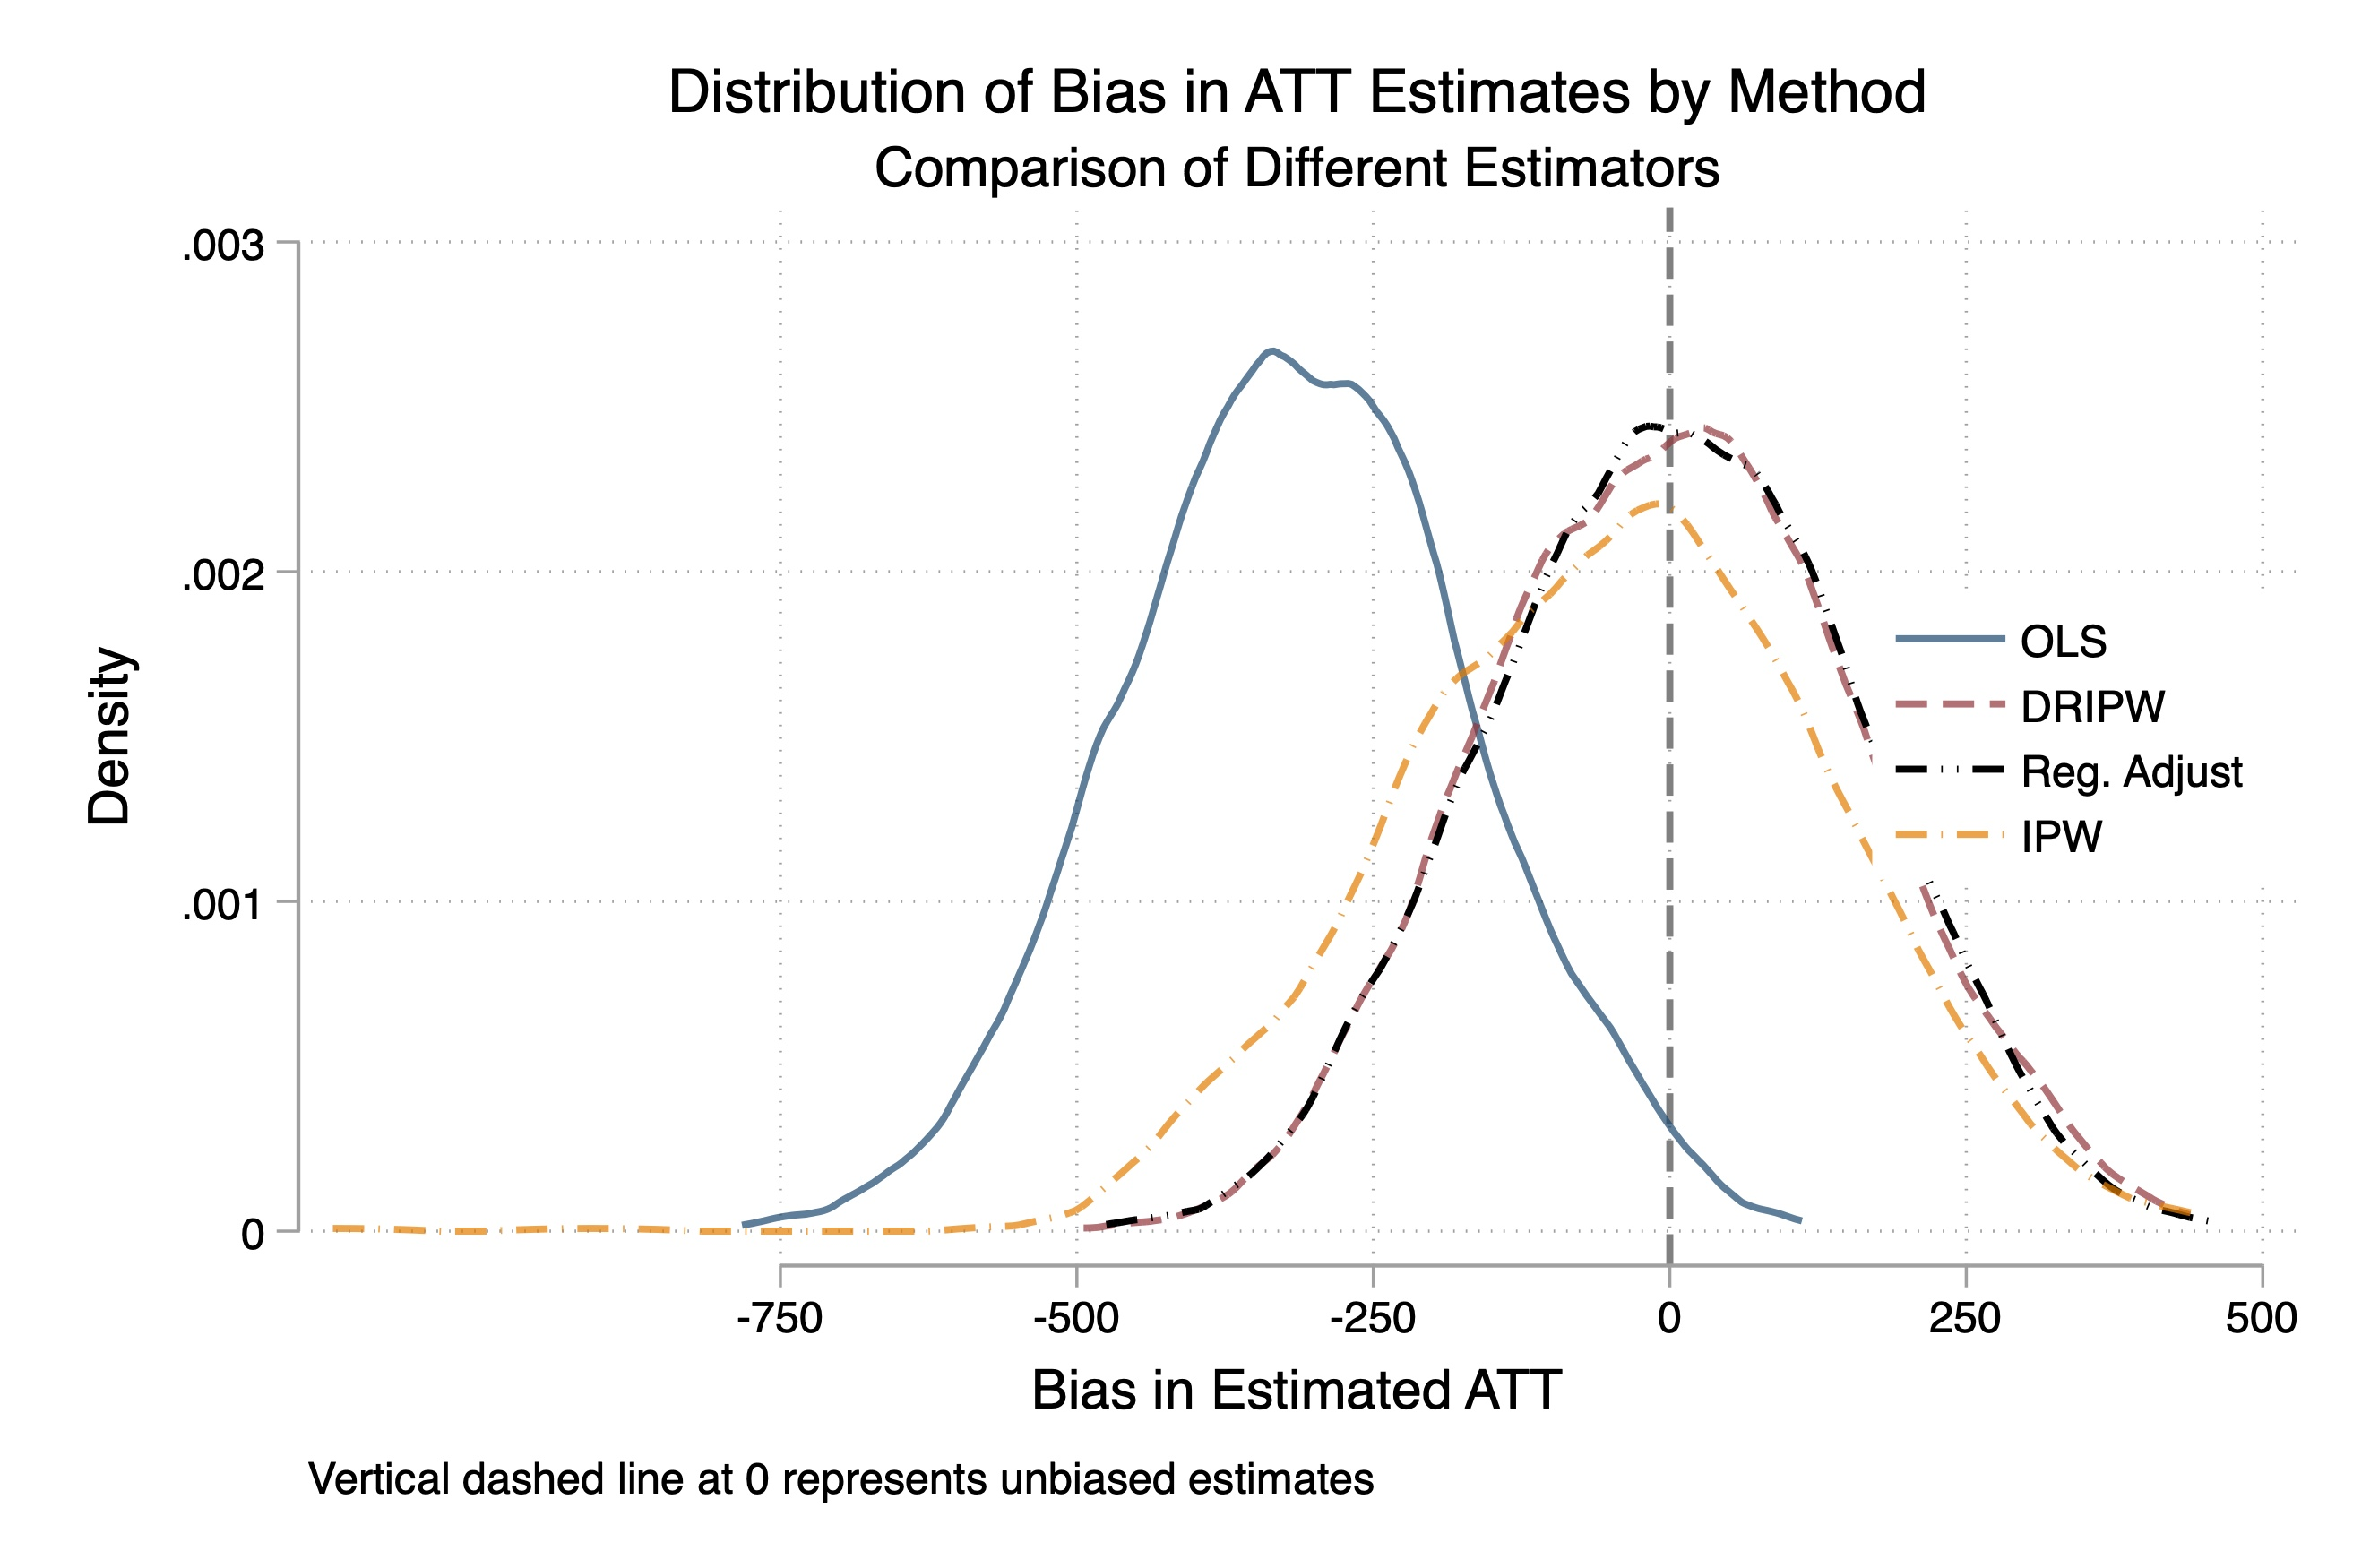
\includegraphics[width=0.6\textwidth]{./lecture_includes/covariates.jpg}
\end{frame}






\end{document}
\begin{frame}{Event studies can mislead}

\begin{itemize}

\item People mistakenly equate parallel trends with parallel pretrends, but you can have one without the other, both or neither
\item One of the ways you can have parallel pre-trends but violate parallel trends is if the trends change differentially by covariate over time (called x-specific trends)
\item Code is called \texttt{misleading_eventstudy.do} and \texttt{misleading_eventstudy.R}
\item Note how well the unconditional parallel trends assumption appears to be when reviewing the graphs only
\end{itemize}

\end{frame}

\begin{frame}{Event studies can mislead}

\begin{figure}
    \centering
    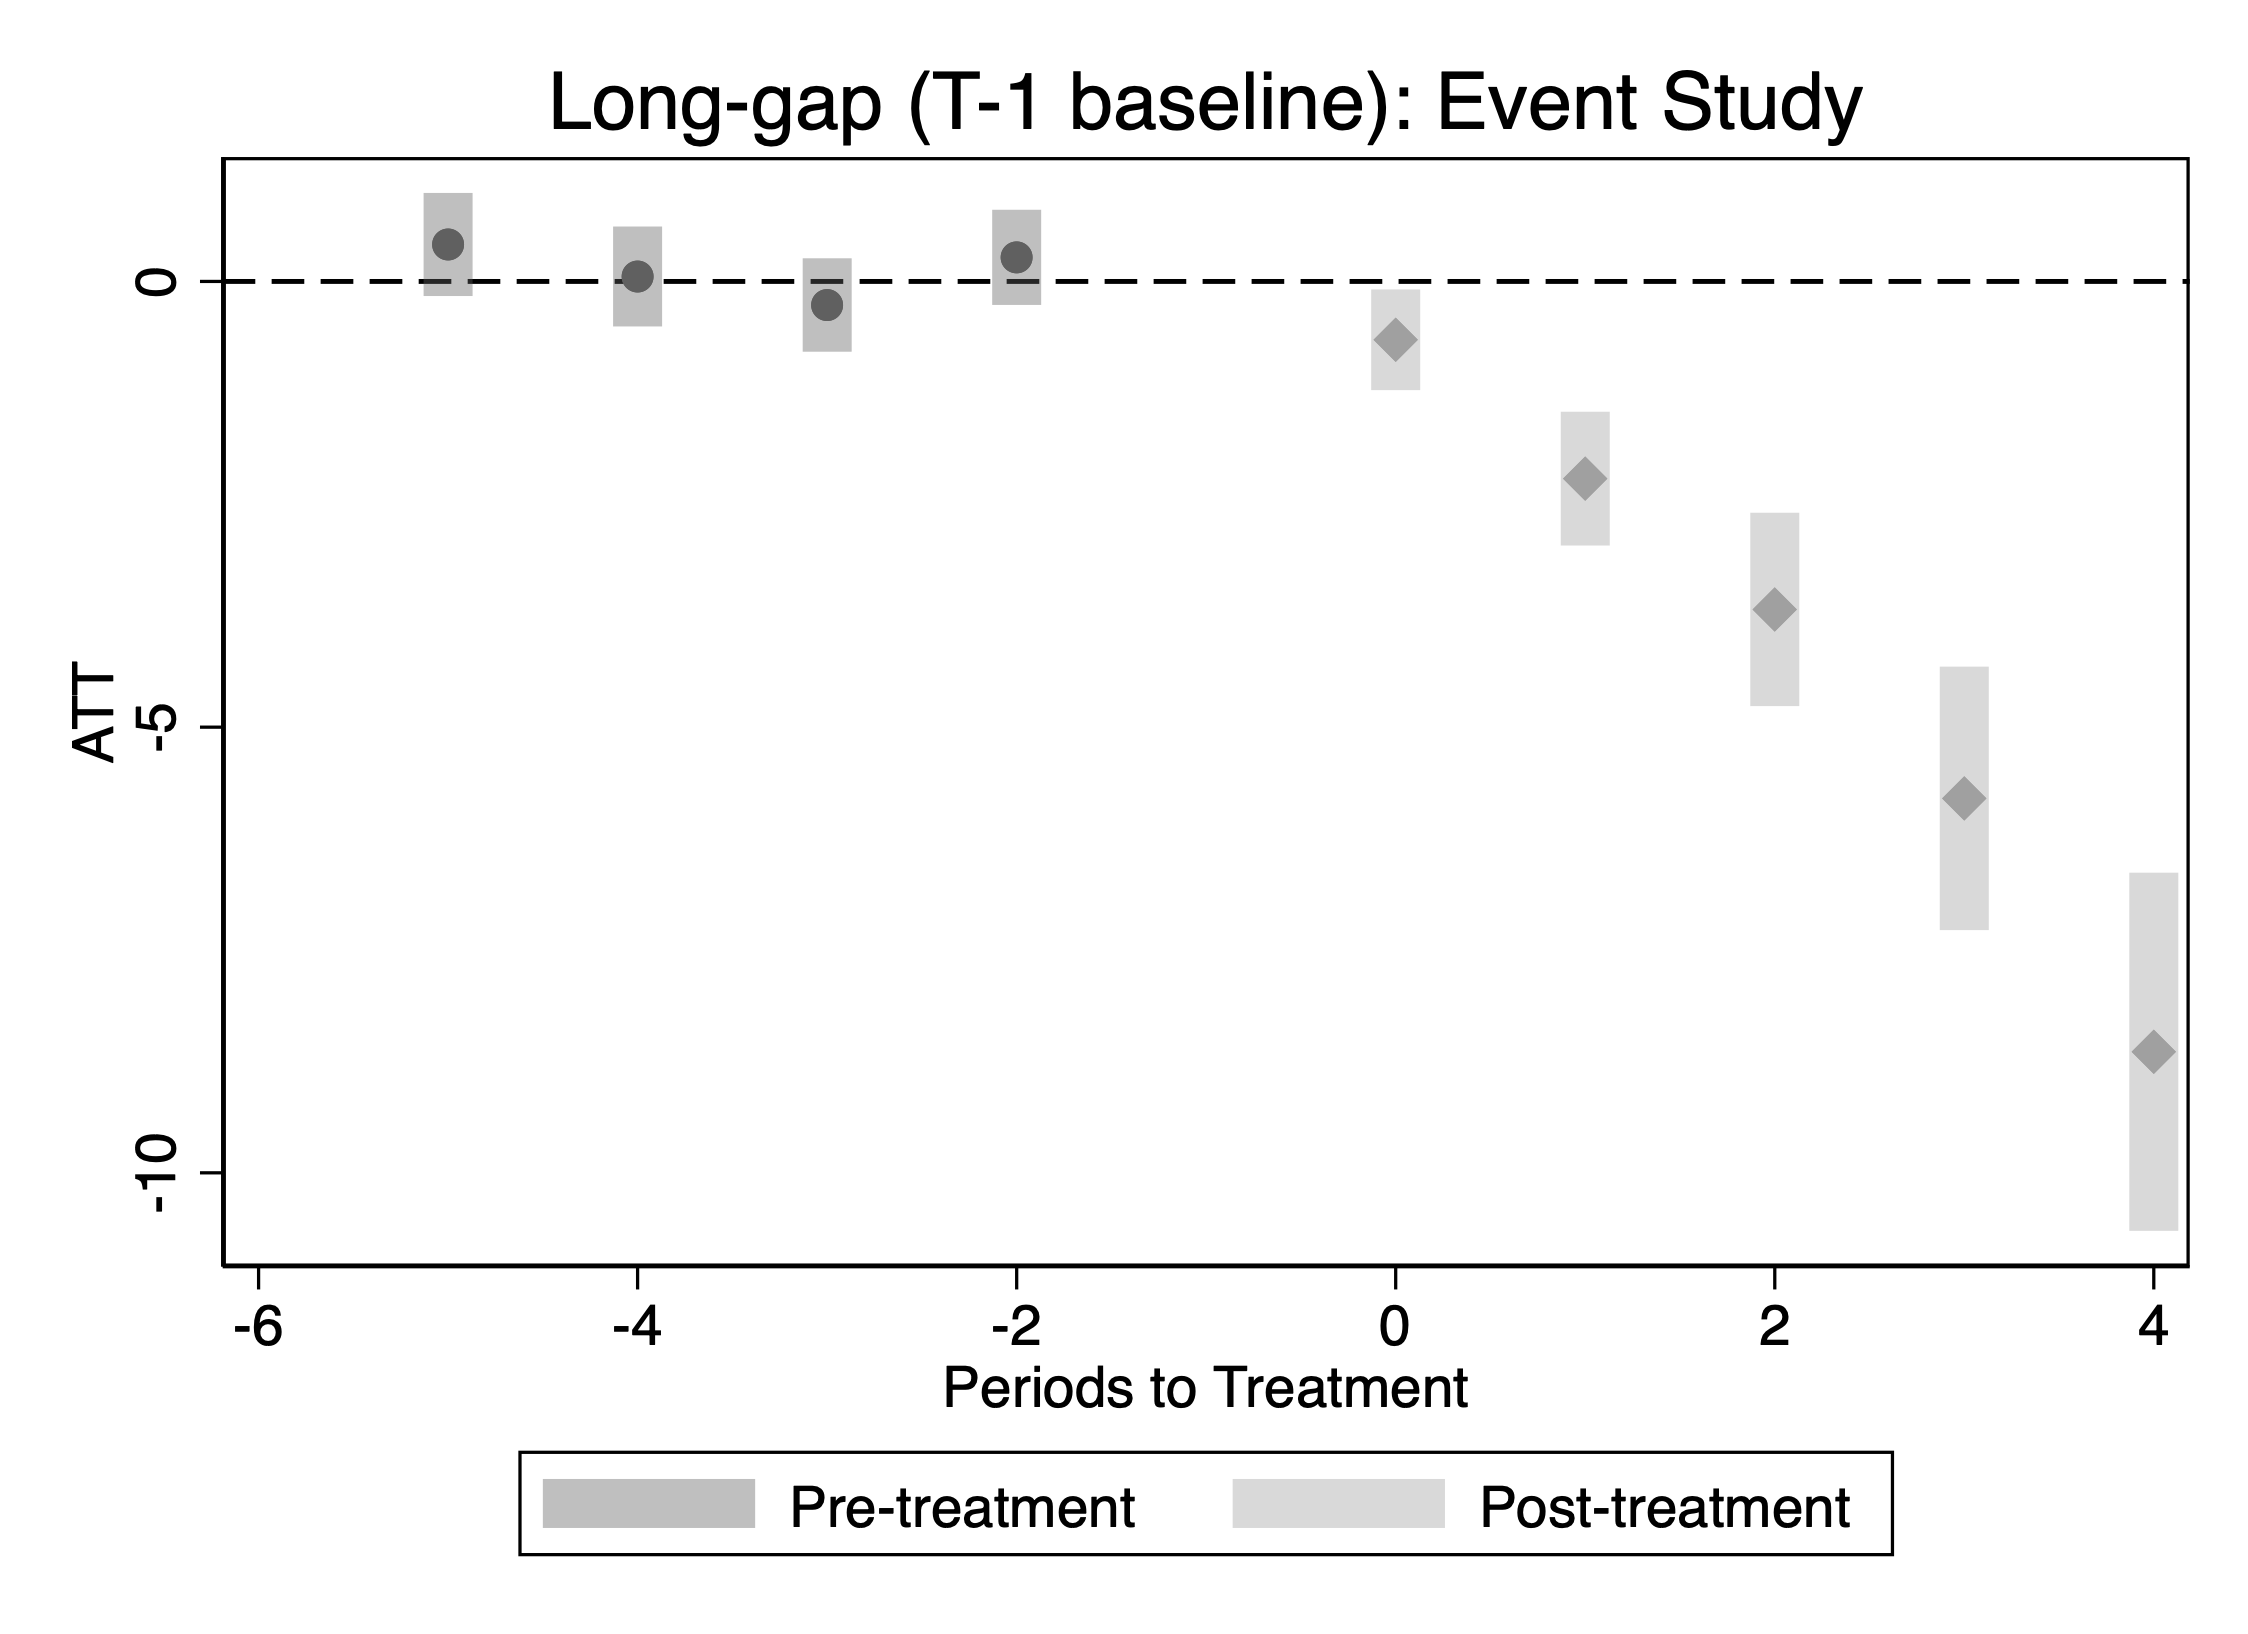
\includegraphics[height=0.75\textheight]{./lecture_includes/es_flawed.png}
\end{figure}

\end{frame}


\begin{frame}{Event studies can mislead}

\begin{figure}
    \centering
    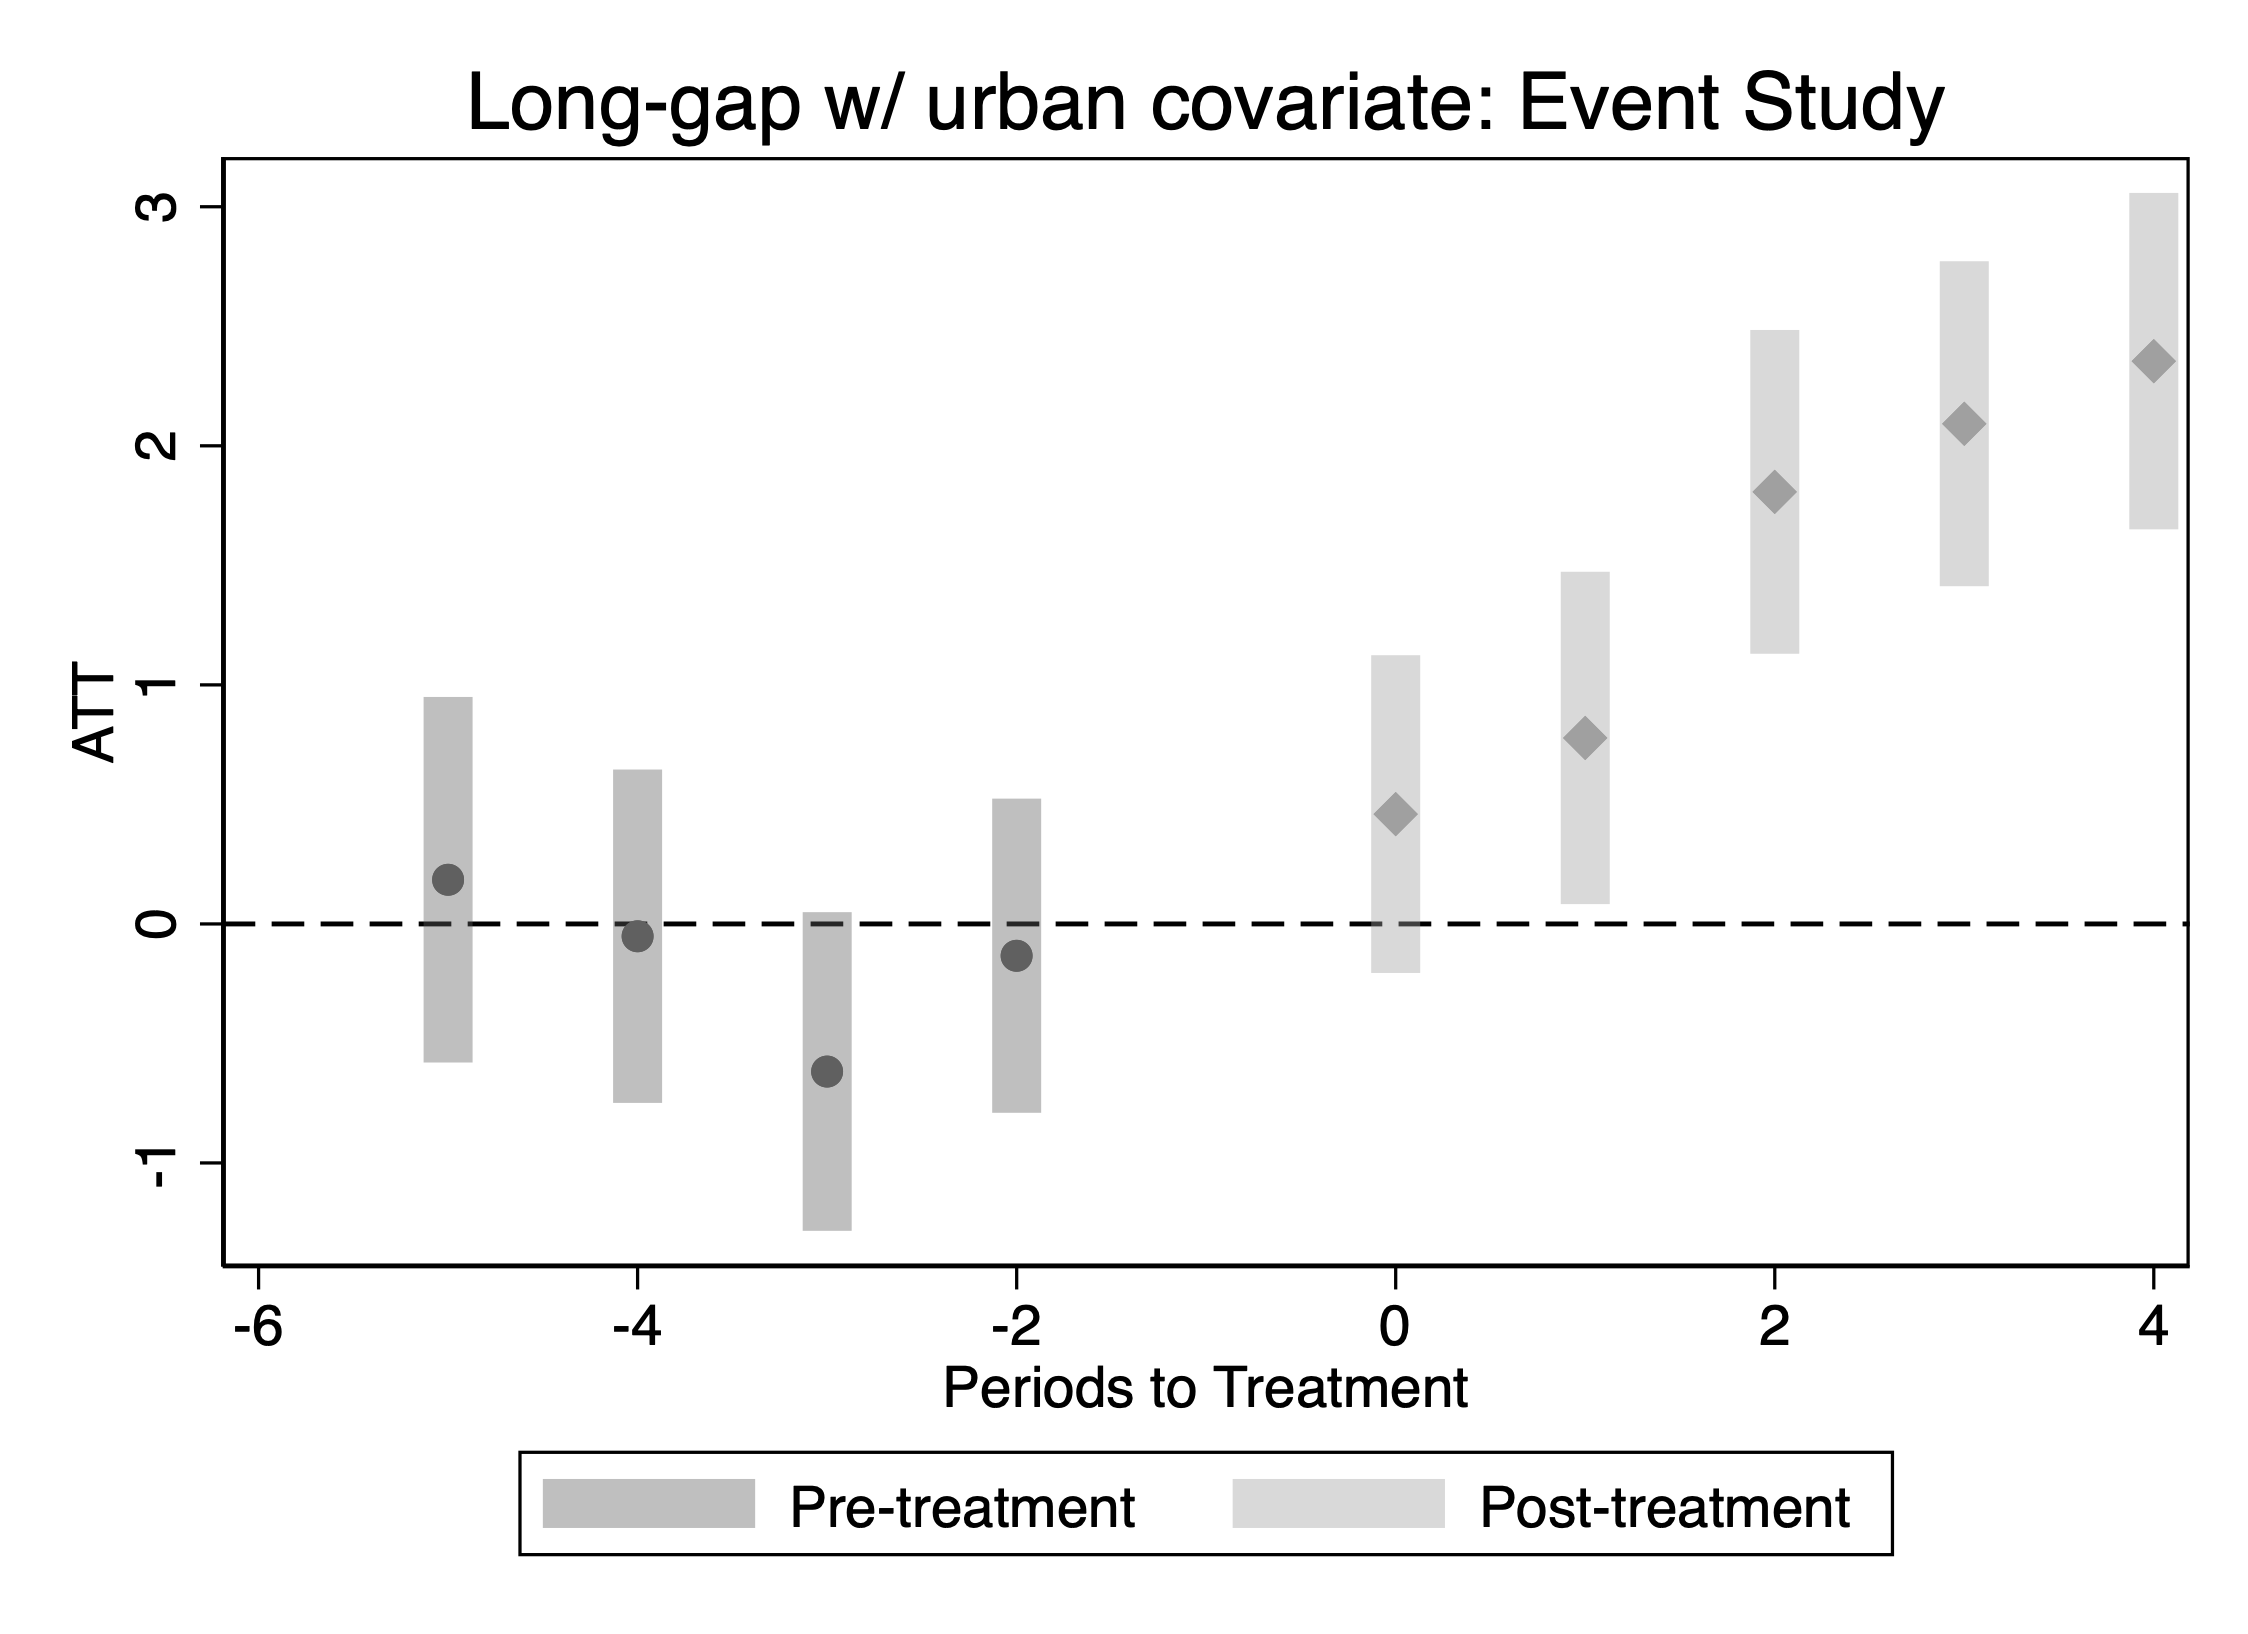
\includegraphics[height=0.75\textheight]{./lecture_includes/es_correct.png}
\end{figure}

\end{frame}

\begin{frame}{Time varying trends in $Y^0$ have \emph{nothing} to do with parallel trends}

\begin{figure}
    \centering
    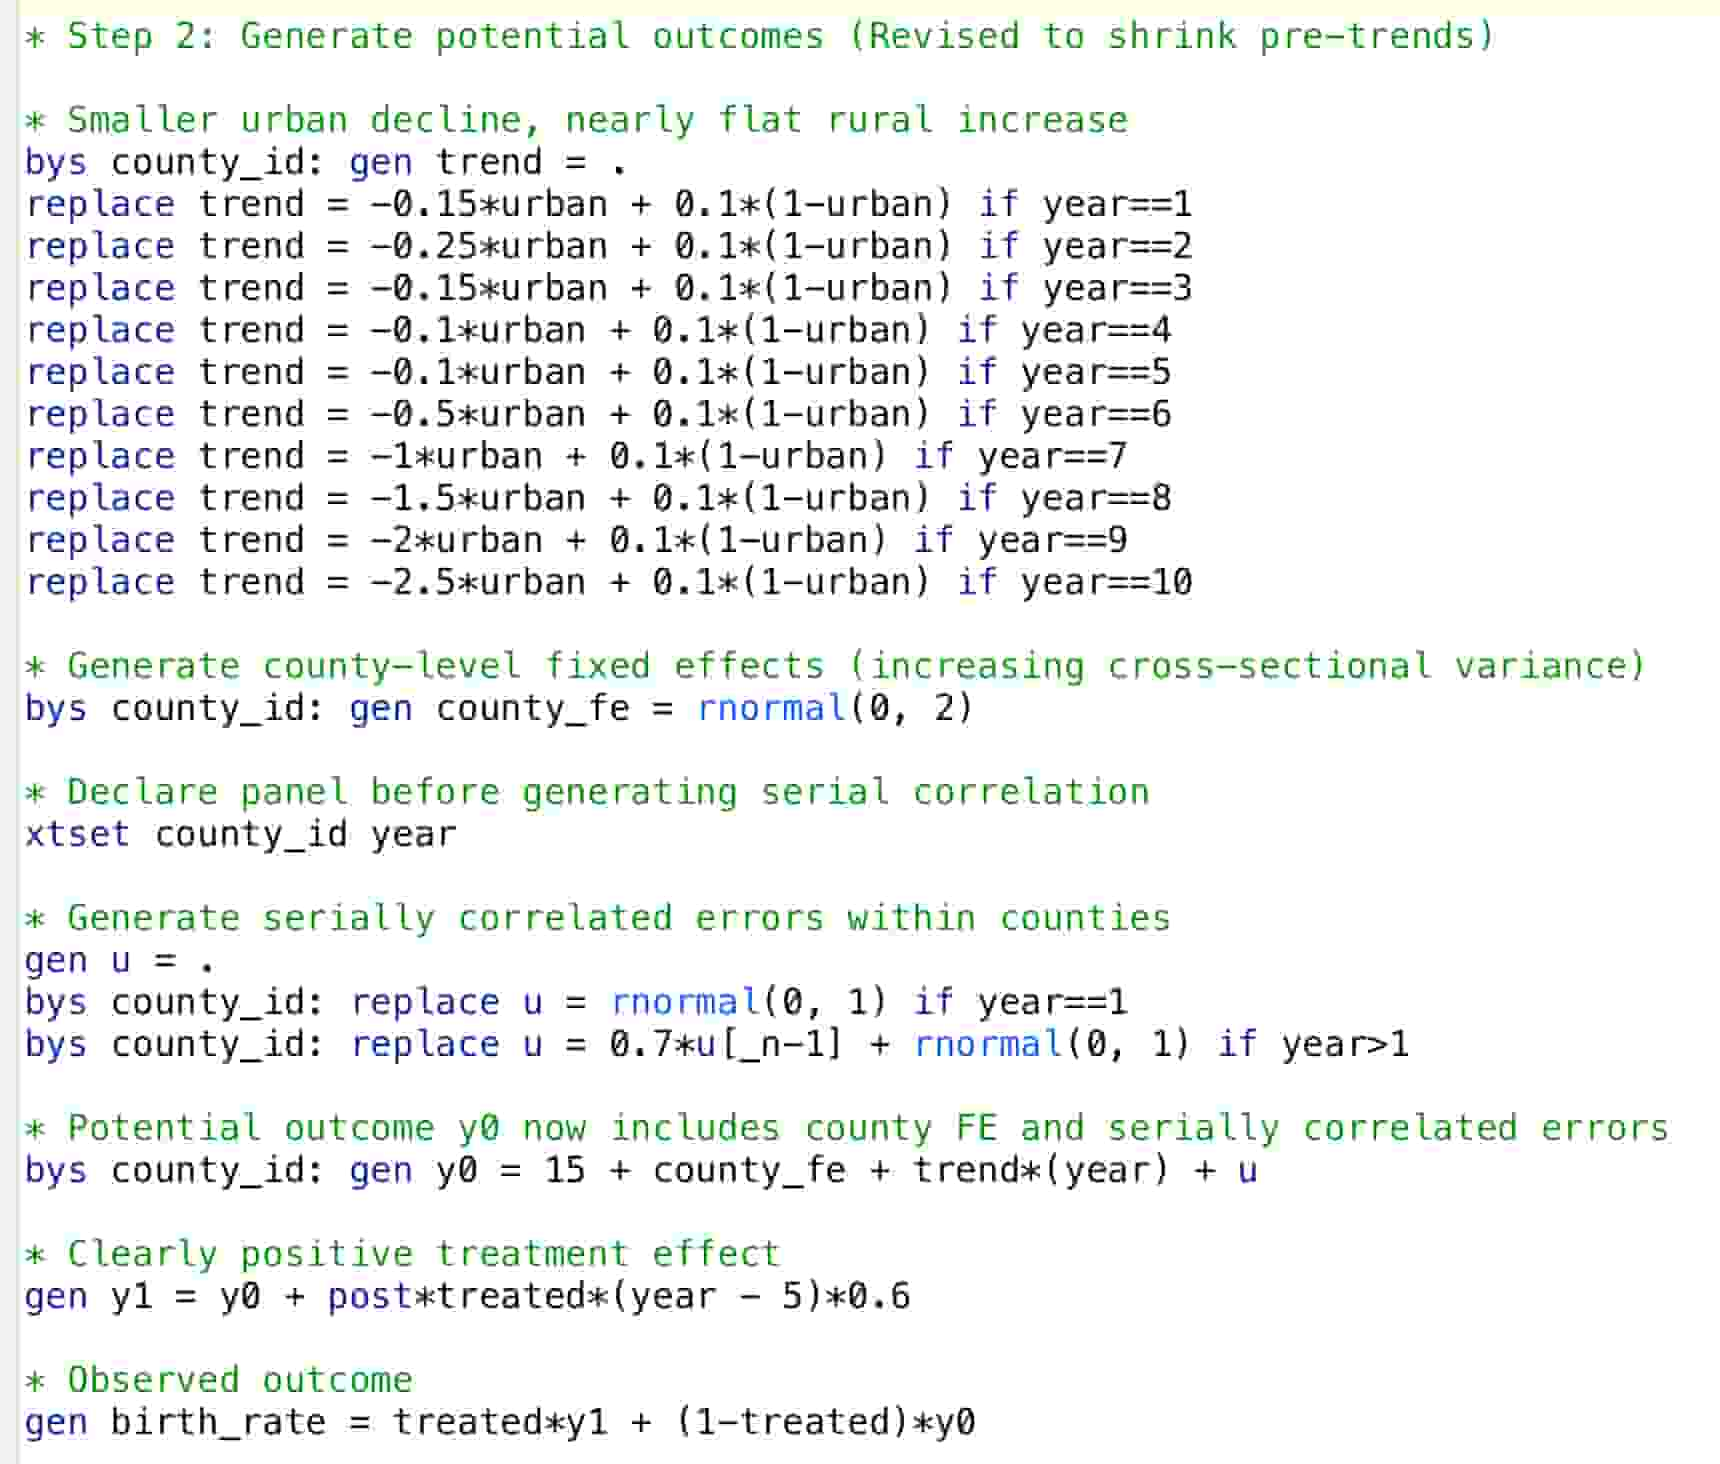
\includegraphics[height=0.75\textheight]{./lecture_includes/misleading_eventstudy_code.jpg}
\end{figure}

\end{frame}

\begin{frame}{Selection can also make event studies misleading}

\begin{itemize}

\item Remember from earlier: some forms of selection that satisfy parallel trends will nonetheless complicate event study plots
\item Selection on baseline $Y^0$, for instance, can cause the pre-trends to break but not parallel trends
\end{itemize}

\end{frame}

\begin{frame}{Selection on $Y^0$ and event studies}

\begin{figure}
    \centering
    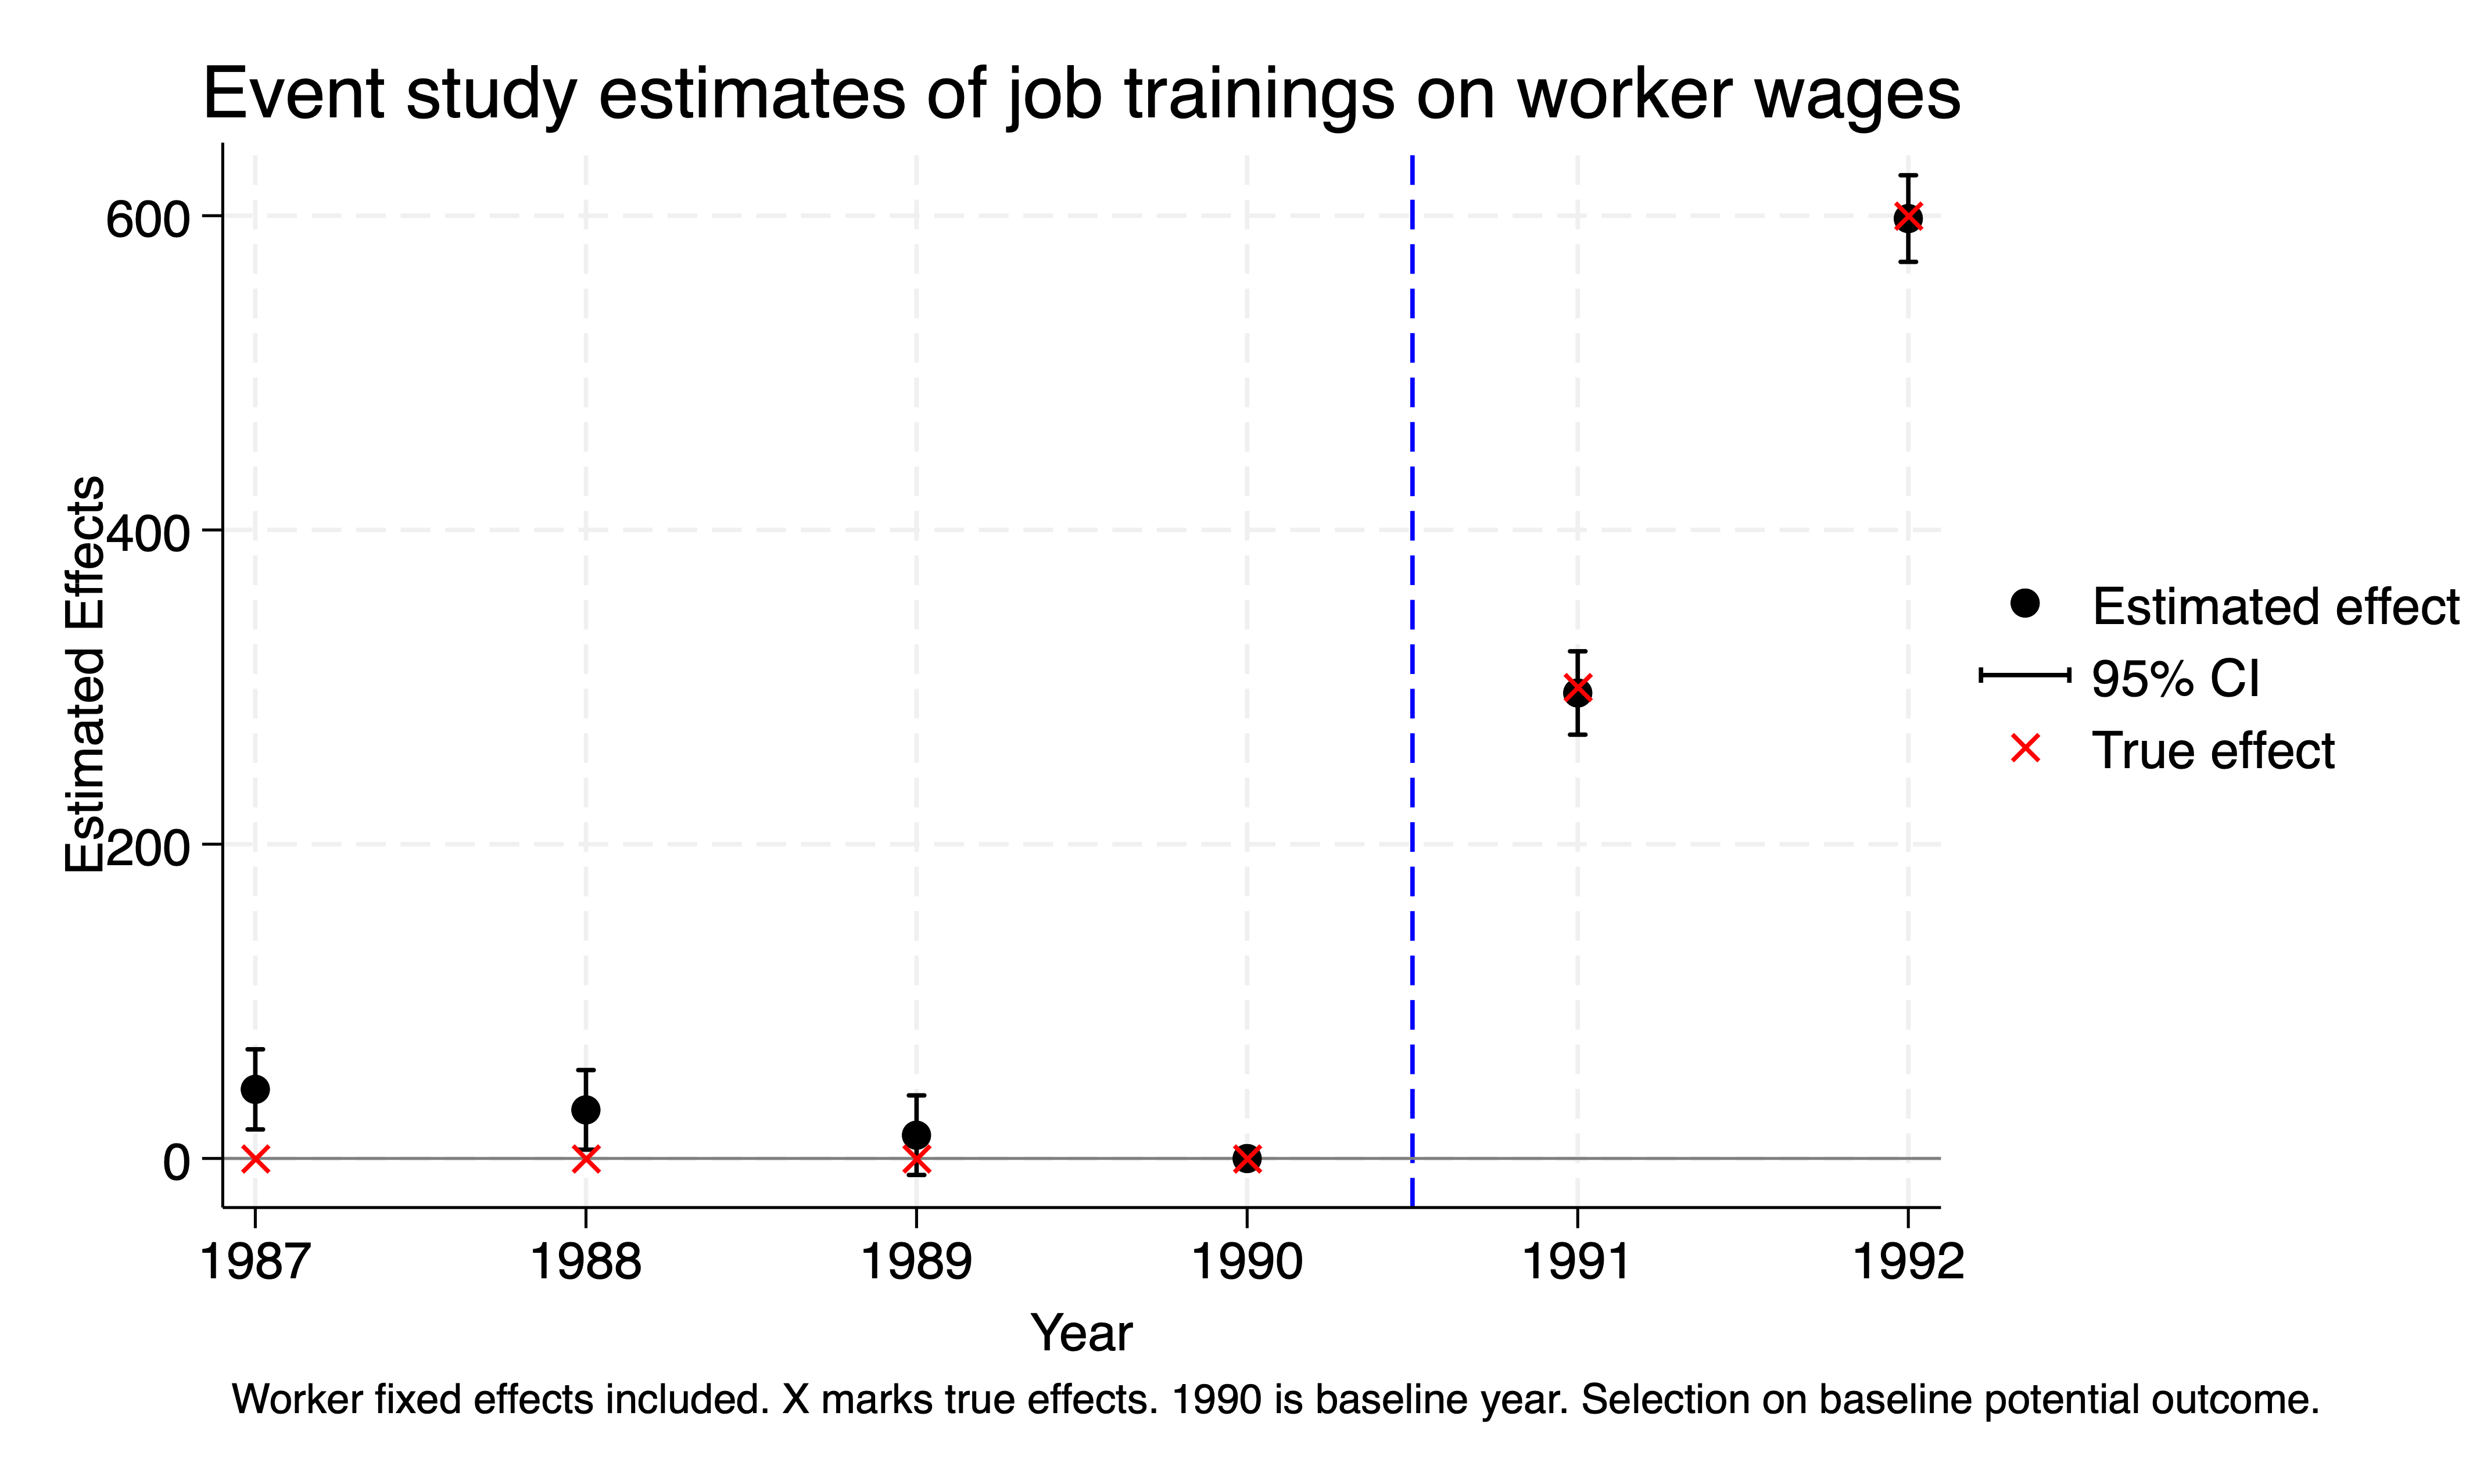
\includegraphics[height=0.70\textheight]{./lecture_includes/selection_y0.png}
\end{figure}

\end{frame}





